\documentclass[twoside]{book}

% Packages required by doxygen
\usepackage{fixltx2e}
\usepackage{calc}
\usepackage{doxygen}
\usepackage[export]{adjustbox} % also loads graphicx
\usepackage{graphicx}
\usepackage[utf8]{inputenc}
\usepackage{makeidx}
\usepackage{multicol}
\usepackage{multirow}
\PassOptionsToPackage{warn}{textcomp}
\usepackage{textcomp}
\usepackage[nointegrals]{wasysym}
\usepackage[table]{xcolor}

% Font selection
\usepackage[T1]{fontenc}
\usepackage[scaled=.90]{helvet}
\usepackage{courier}
\usepackage{amssymb}
\usepackage{sectsty}
\renewcommand{\familydefault}{\sfdefault}
\allsectionsfont{%
  \fontseries{bc}\selectfont%
  \color{darkgray}%
}
\renewcommand{\DoxyLabelFont}{%
  \fontseries{bc}\selectfont%
  \color{darkgray}%
}
\newcommand{\+}{\discretionary{\mbox{\scriptsize$\hookleftarrow$}}{}{}}

% Page & text layout
\usepackage{geometry}
\geometry{%
  a4paper,%
  top=2.5cm,%
  bottom=2.5cm,%
  left=2.5cm,%
  right=2.5cm%
}
\tolerance=750
\hfuzz=15pt
\hbadness=750
\setlength{\emergencystretch}{15pt}
\setlength{\parindent}{0cm}
\setlength{\parskip}{3ex plus 2ex minus 2ex}
\makeatletter
\renewcommand{\paragraph}{%
  \@startsection{paragraph}{4}{0ex}{-1.0ex}{1.0ex}{%
    \normalfont\normalsize\bfseries\SS@parafont%
  }%
}
\renewcommand{\subparagraph}{%
  \@startsection{subparagraph}{5}{0ex}{-1.0ex}{1.0ex}{%
    \normalfont\normalsize\bfseries\SS@subparafont%
  }%
}
\makeatother

% Headers & footers
\usepackage{fancyhdr}
\pagestyle{fancyplain}
\fancyhead[LE]{\fancyplain{}{\bfseries\thepage}}
\fancyhead[CE]{\fancyplain{}{}}
\fancyhead[RE]{\fancyplain{}{\bfseries\leftmark}}
\fancyhead[LO]{\fancyplain{}{\bfseries\rightmark}}
\fancyhead[CO]{\fancyplain{}{}}
\fancyhead[RO]{\fancyplain{}{\bfseries\thepage}}
\fancyfoot[LE]{\fancyplain{}{}}
\fancyfoot[CE]{\fancyplain{}{}}
\fancyfoot[RE]{\fancyplain{}{\bfseries\scriptsize Generated by Doxygen }}
\fancyfoot[LO]{\fancyplain{}{\bfseries\scriptsize Generated by Doxygen }}
\fancyfoot[CO]{\fancyplain{}{}}
\fancyfoot[RO]{\fancyplain{}{}}
\renewcommand{\footrulewidth}{0.4pt}
\renewcommand{\chaptermark}[1]{%
  \markboth{#1}{}%
}
\renewcommand{\sectionmark}[1]{%
  \markright{\thesection\ #1}%
}

% Indices & bibliography
\usepackage{natbib}
\usepackage[titles]{tocloft}
\setcounter{tocdepth}{3}
\setcounter{secnumdepth}{5}
\makeindex

% Hyperlinks (required, but should be loaded last)
\usepackage{ifpdf}
\ifpdf
  \usepackage[pdftex,pagebackref=true]{hyperref}
\else
  \usepackage[ps2pdf,pagebackref=true]{hyperref}
\fi
\hypersetup{%
  colorlinks=true,%
  linkcolor=blue,%
  citecolor=blue,%
  unicode%
}

% Custom commands
\newcommand{\clearemptydoublepage}{%
  \newpage{\pagestyle{empty}\cleardoublepage}%
}

\usepackage{caption}
\captionsetup{labelsep=space,justification=centering,font={bf},singlelinecheck=off,skip=4pt,position=top}

%===== C O N T E N T S =====

\begin{document}

% Titlepage & ToC
\hypersetup{pageanchor=false,
             bookmarksnumbered=true,
             pdfencoding=unicode
            }
\pagenumbering{alph}
\begin{titlepage}
\vspace*{7cm}
\begin{center}%
{\Large sw\+\_\+engineering\+\_\+hw3 }\\
\vspace*{1cm}
{\large Generated by Doxygen 1.8.14}\\
\end{center}
\end{titlepage}
\clearemptydoublepage
\pagenumbering{roman}
\tableofcontents
\clearemptydoublepage
\pagenumbering{arabic}
\hypersetup{pageanchor=true}

%--- Begin generated contents ---
\chapter{Hierarchical Index}
\section{Class Hierarchy}
This inheritance list is sorted roughly, but not completely, alphabetically\+:\begin{DoxyCompactList}
\item \contentsline{section}{Abstract\+Boundary}{\pageref{class_abstract_boundary}}{}
\begin{DoxyCompactList}
\item \contentsline{section}{add\+Accommodation\+UI}{\pageref{classadd_accommodation_u_i}}{}
\item \contentsline{section}{List\+Host\+Accommodation\+UI}{\pageref{class_list_host_accommodation_u_i}}{}
\item \contentsline{section}{Login\+UI}{\pageref{class_login_u_i}}{}
\item \contentsline{section}{Logout\+UI}{\pageref{class_logout_u_i}}{}
\item \contentsline{section}{Opaque\+Inventory\+UI}{\pageref{class_opaque_inventory_u_i}}{}
\item \contentsline{section}{Register\+UI}{\pageref{class_register_u_i}}{}
\item \contentsline{section}{Search\+Reservation\+UI}{\pageref{class_search_reservation_u_i}}{}
\item \contentsline{section}{Search\+UI}{\pageref{class_search_u_i}}{}
\item \contentsline{section}{Session\+UI}{\pageref{class_session_u_i}}{}
\item \contentsline{section}{Withdrawal\+UI}{\pageref{class_withdrawal_u_i}}{}
\end{DoxyCompactList}
\item \contentsline{section}{Abstract\+Control}{\pageref{class_abstract_control}}{}
\begin{DoxyCompactList}
\item \contentsline{section}{add\+Accommodation}{\pageref{classadd_accommodation}}{}
\item \contentsline{section}{List\+Host\+Accommodation\+Control}{\pageref{class_list_host_accommodation_control}}{}
\item \contentsline{section}{Login\+Control}{\pageref{class_login_control}}{}
\item \contentsline{section}{Logout\+Control}{\pageref{class_logout_control}}{}
\item \contentsline{section}{Opaque\+Inventory\+Control}{\pageref{class_opaque_inventory_control}}{}
\item \contentsline{section}{Register\+Control}{\pageref{class_register_control}}{}
\item \contentsline{section}{Search\+Control}{\pageref{class_search_control}}{}
\item \contentsline{section}{Search\+Reservation\+Control}{\pageref{class_search_reservation_control}}{}
\item \contentsline{section}{Session\+Control}{\pageref{class_session_control}}{}
\item \contentsline{section}{Withdrawal\+Control}{\pageref{class_withdrawal_control}}{}
\end{DoxyCompactList}
\item \contentsline{section}{Accommodation}{\pageref{class_accommodation}}{}
\item \contentsline{section}{Collection$<$ T $>$}{\pageref{class_collection}}{}
\item \contentsline{section}{Collection$<$ Accommodation $>$}{\pageref{class_collection}}{}
\begin{DoxyCompactList}
\item \contentsline{section}{Accommodation\+Collection}{\pageref{class_accommodation_collection}}{}
\end{DoxyCompactList}
\item \contentsline{section}{Collection$<$ Member $>$}{\pageref{class_collection}}{}
\begin{DoxyCompactList}
\item \contentsline{section}{Member\+Collection}{\pageref{class_member_collection}}{}
\end{DoxyCompactList}
\item \contentsline{section}{Collection$<$ Reservation $>$}{\pageref{class_collection}}{}
\begin{DoxyCompactList}
\item \contentsline{section}{Reservation\+Collection}{\pageref{class_reservation_collection}}{}
\end{DoxyCompactList}
\item \contentsline{section}{Collection$<$ Session $>$}{\pageref{class_collection}}{}
\begin{DoxyCompactList}
\item \contentsline{section}{Session\+Collection}{\pageref{class_session_collection}}{}
\end{DoxyCompactList}
\item \contentsline{section}{Date\+Time\+Utils}{\pageref{class_date_time_utils}}{}
\item \contentsline{section}{Member}{\pageref{class_member}}{}
\begin{DoxyCompactList}
\item \contentsline{section}{Guest}{\pageref{class_guest}}{}
\item \contentsline{section}{Host}{\pageref{class_host}}{}
\end{DoxyCompactList}
\item \contentsline{section}{Opaque}{\pageref{class_opaque}}{}
\item \contentsline{section}{Output\+Writer}{\pageref{class_output_writer}}{}
\item \contentsline{section}{Reservation}{\pageref{class_reservation}}{}
\item \contentsline{section}{Session}{\pageref{class_session}}{}
\item \contentsline{section}{Time}{\pageref{class_time}}{}
\end{DoxyCompactList}

\chapter{Class Index}
\section{Class List}
Here are the classes, structs, unions and interfaces with brief descriptions\+:\begin{DoxyCompactList}
\item\contentsline{section}{\mbox{\hyperlink{class_abstract_boundary}{Abstract\+Boundary}} }{\pageref{class_abstract_boundary}}{}
\item\contentsline{section}{\mbox{\hyperlink{class_abstract_control}{Abstract\+Control}} }{\pageref{class_abstract_control}}{}
\item\contentsline{section}{\mbox{\hyperlink{class_accommodation}{Accommodation}} }{\pageref{class_accommodation}}{}
\item\contentsline{section}{\mbox{\hyperlink{class_accommodation_collection}{Accommodation\+Collection}} }{\pageref{class_accommodation_collection}}{}
\item\contentsline{section}{\mbox{\hyperlink{classadd_accommodation}{add\+Accommodation}} }{\pageref{classadd_accommodation}}{}
\item\contentsline{section}{\mbox{\hyperlink{classadd_accommodation_u_i}{add\+Accommodation\+UI}} }{\pageref{classadd_accommodation_u_i}}{}
\item\contentsline{section}{\mbox{\hyperlink{class_collection}{Collection$<$ T $>$}} }{\pageref{class_collection}}{}
\item\contentsline{section}{\mbox{\hyperlink{class_date_time_utils}{Date\+Time\+Utils}} }{\pageref{class_date_time_utils}}{}
\item\contentsline{section}{\mbox{\hyperlink{class_guest}{Guest}} }{\pageref{class_guest}}{}
\item\contentsline{section}{\mbox{\hyperlink{class_host}{Host}} }{\pageref{class_host}}{}
\item\contentsline{section}{\mbox{\hyperlink{class_list_host_accommodation_control}{List\+Host\+Accommodation\+Control}} }{\pageref{class_list_host_accommodation_control}}{}
\item\contentsline{section}{\mbox{\hyperlink{class_list_host_accommodation_u_i}{List\+Host\+Accommodation\+UI}} }{\pageref{class_list_host_accommodation_u_i}}{}
\item\contentsline{section}{\mbox{\hyperlink{class_login_control}{Login\+Control}} }{\pageref{class_login_control}}{}
\item\contentsline{section}{\mbox{\hyperlink{class_login_u_i}{Login\+UI}} }{\pageref{class_login_u_i}}{}
\item\contentsline{section}{\mbox{\hyperlink{class_logout_control}{Logout\+Control}} }{\pageref{class_logout_control}}{}
\item\contentsline{section}{\mbox{\hyperlink{class_logout_u_i}{Logout\+UI}} }{\pageref{class_logout_u_i}}{}
\item\contentsline{section}{\mbox{\hyperlink{class_member}{Member}} }{\pageref{class_member}}{}
\item\contentsline{section}{\mbox{\hyperlink{class_member_collection}{Member\+Collection}} }{\pageref{class_member_collection}}{}
\item\contentsline{section}{\mbox{\hyperlink{class_opaque}{Opaque}} }{\pageref{class_opaque}}{}
\item\contentsline{section}{\mbox{\hyperlink{class_opaque_inventory_control}{Opaque\+Inventory\+Control}} }{\pageref{class_opaque_inventory_control}}{}
\item\contentsline{section}{\mbox{\hyperlink{class_opaque_inventory_u_i}{Opaque\+Inventory\+UI}} }{\pageref{class_opaque_inventory_u_i}}{}
\item\contentsline{section}{\mbox{\hyperlink{class_output_writer}{Output\+Writer}} }{\pageref{class_output_writer}}{}
\item\contentsline{section}{\mbox{\hyperlink{class_register_control}{Register\+Control}} }{\pageref{class_register_control}}{}
\item\contentsline{section}{\mbox{\hyperlink{class_register_u_i}{Register\+UI}} }{\pageref{class_register_u_i}}{}
\item\contentsline{section}{\mbox{\hyperlink{class_reservation}{Reservation}} }{\pageref{class_reservation}}{}
\item\contentsline{section}{\mbox{\hyperlink{class_reservation_collection}{Reservation\+Collection}} }{\pageref{class_reservation_collection}}{}
\item\contentsline{section}{\mbox{\hyperlink{class_search_control}{Search\+Control}} }{\pageref{class_search_control}}{}
\item\contentsline{section}{\mbox{\hyperlink{class_search_reservation_control}{Search\+Reservation\+Control}} }{\pageref{class_search_reservation_control}}{}
\item\contentsline{section}{\mbox{\hyperlink{class_search_reservation_u_i}{Search\+Reservation\+UI}} }{\pageref{class_search_reservation_u_i}}{}
\item\contentsline{section}{\mbox{\hyperlink{class_search_u_i}{Search\+UI}} }{\pageref{class_search_u_i}}{}
\item\contentsline{section}{\mbox{\hyperlink{class_session}{Session}} }{\pageref{class_session}}{}
\item\contentsline{section}{\mbox{\hyperlink{class_session_collection}{Session\+Collection}} }{\pageref{class_session_collection}}{}
\item\contentsline{section}{\mbox{\hyperlink{class_session_control}{Session\+Control}} }{\pageref{class_session_control}}{}
\item\contentsline{section}{\mbox{\hyperlink{class_session_u_i}{Session\+UI}} }{\pageref{class_session_u_i}}{}
\item\contentsline{section}{\mbox{\hyperlink{class_time}{Time}} }{\pageref{class_time}}{}
\item\contentsline{section}{\mbox{\hyperlink{class_withdrawal_control}{Withdrawal\+Control}} }{\pageref{class_withdrawal_control}}{}
\item\contentsline{section}{\mbox{\hyperlink{class_withdrawal_u_i}{Withdrawal\+UI}} }{\pageref{class_withdrawal_u_i}}{}
\end{DoxyCompactList}

\chapter{Class Documentation}
\hypertarget{class_abstract_boundary}{}\section{Abstract\+Boundary Class Reference}
\label{class_abstract_boundary}\index{Abstract\+Boundary@{Abstract\+Boundary}}
Inheritance diagram for Abstract\+Boundary\+:\begin{figure}[H]
\begin{center}
\leavevmode
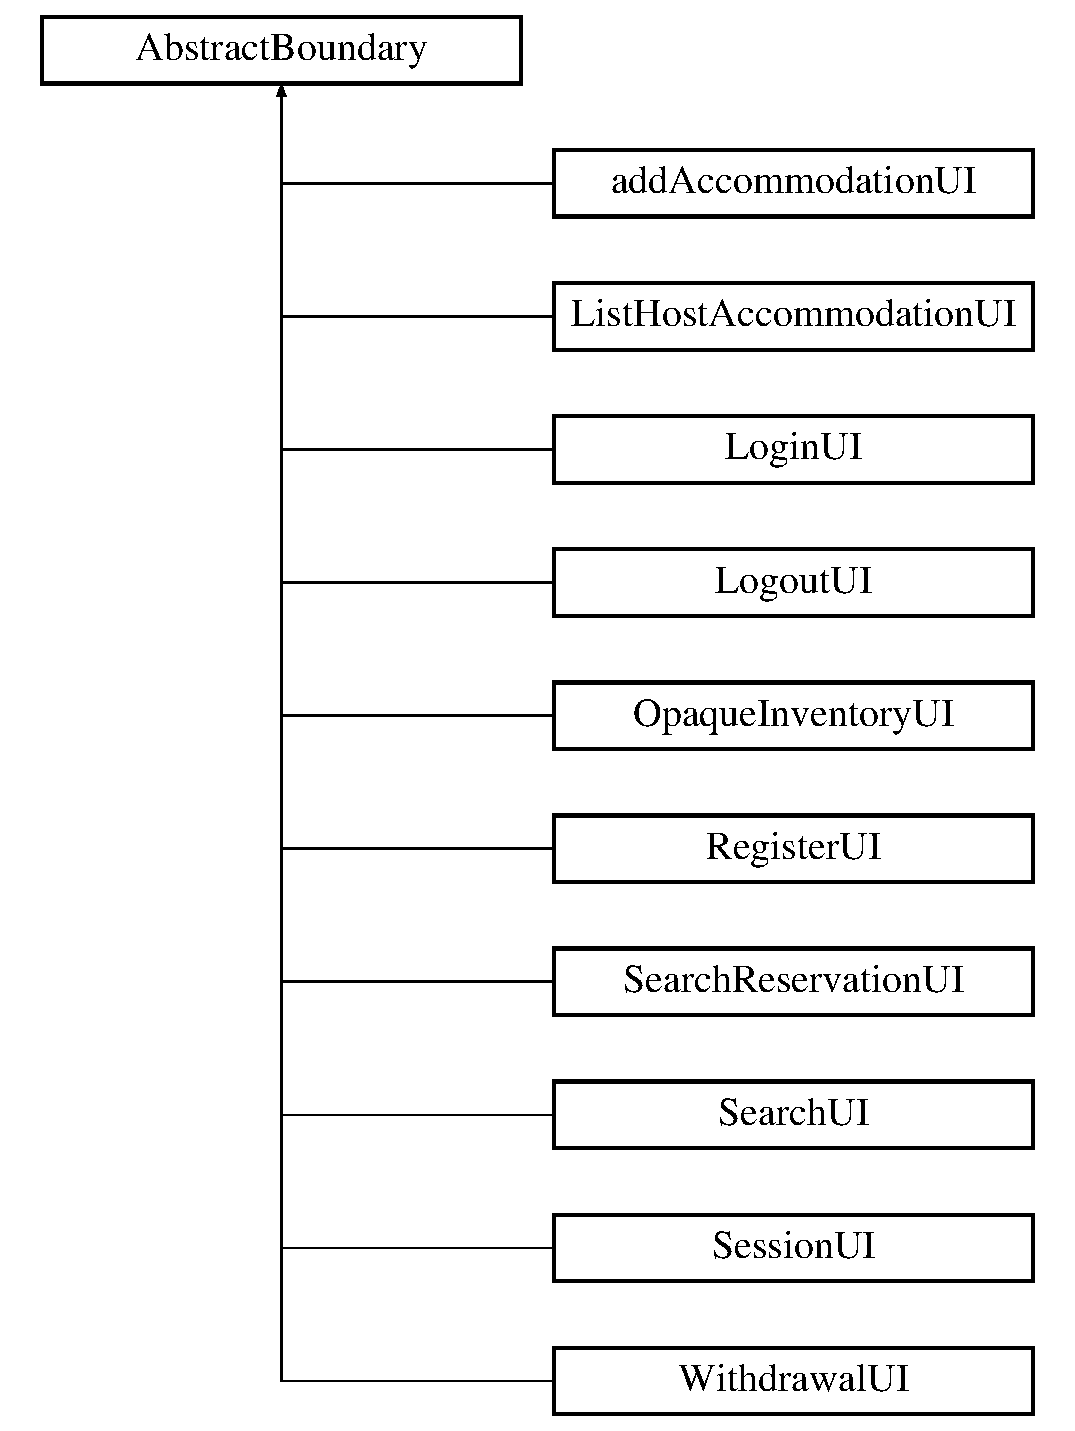
\includegraphics[height=11.000000cm]{class_abstract_boundary}
\end{center}
\end{figure}
\subsection*{Public Member Functions}
\begin{DoxyCompactItemize}
\item 
\mbox{\Hypertarget{class_abstract_boundary_a58d0f5dad1635f64f847d96f3451b145}\label{class_abstract_boundary_a58d0f5dad1635f64f847d96f3451b145}} 
virtual void {\bfseries print} (const char $\ast$fmt,...)
\item 
\mbox{\Hypertarget{class_abstract_boundary_a70c2c2983a38d43a6c5ccd6e831d5c5d}\label{class_abstract_boundary_a70c2c2983a38d43a6c5ccd6e831d5c5d}} 
virtual void {\bfseries print\+Line} (const char $\ast$fmt,...)
\end{DoxyCompactItemize}
\subsection*{Protected Member Functions}
\begin{DoxyCompactItemize}
\item 
\mbox{\Hypertarget{class_abstract_boundary_ae5d219b7f0f0941db96fb033469e7593}\label{class_abstract_boundary_ae5d219b7f0f0941db96fb033469e7593}} 
\mbox{\hyperlink{class_abstract_control}{Abstract\+Control}} $\ast$ {\bfseries get\+Control} ()
\end{DoxyCompactItemize}
\subsection*{Friends}
\begin{DoxyCompactItemize}
\item 
\mbox{\Hypertarget{class_abstract_boundary_a53e200cea9e8515d1a76f980bcfd500d}\label{class_abstract_boundary_a53e200cea9e8515d1a76f980bcfd500d}} 
class {\bfseries Abstract\+Control}
\end{DoxyCompactItemize}


The documentation for this class was generated from the following files\+:\begin{DoxyCompactItemize}
\item 
src/boundaries/Abstract\+Boundary.\+h\item 
src/boundaries/Abstract\+Boundary.\+cpp\end{DoxyCompactItemize}

\hypertarget{class_abstract_control}{}\section{Abstract\+Control Class Reference}
\label{class_abstract_control}\index{Abstract\+Control@{Abstract\+Control}}


{\ttfamily \#include $<$Abstract\+Control.\+h$>$}

Inheritance diagram for Abstract\+Control\+:\begin{figure}[H]
\begin{center}
\leavevmode
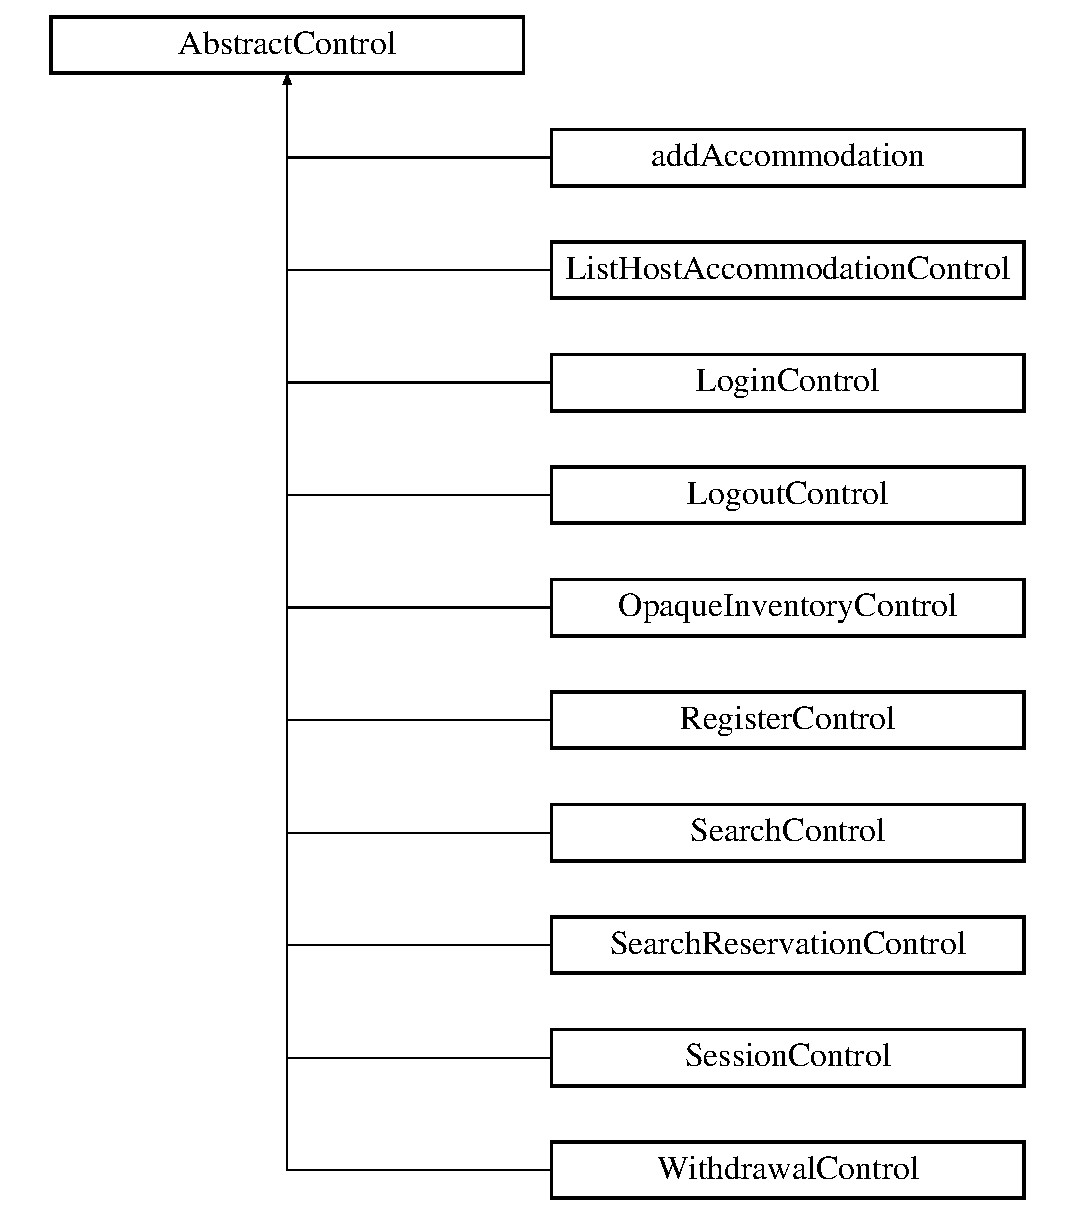
\includegraphics[height=11.000000cm]{class_abstract_control}
\end{center}
\end{figure}
\subsection*{Public Member Functions}
\begin{DoxyCompactItemize}
\item 
\mbox{\Hypertarget{class_abstract_control_a01dbe49782ca39665619e8d254d9df7f}\label{class_abstract_control_a01dbe49782ca39665619e8d254d9df7f}} 
\mbox{\hyperlink{class_abstract_boundary}{Abstract\+Boundary}} $\ast$ {\bfseries get\+Boundary} ()
\item 
\mbox{\Hypertarget{class_abstract_control_a8d4de279a0a6209c60ca14678507d993}\label{class_abstract_control_a8d4de279a0a6209c60ca14678507d993}} 
\mbox{\hyperlink{class_member}{Member}} $\ast$ {\bfseries get\+Current\+Member} ()
\end{DoxyCompactItemize}
\subsection*{Protected Member Functions}
\begin{DoxyCompactItemize}
\item 
\mbox{\Hypertarget{class_abstract_control_aa762455bc70bbb9b065ef6c8715ec2e4}\label{class_abstract_control_aa762455bc70bbb9b065ef6c8715ec2e4}} 
{\bfseries Abstract\+Control} (\mbox{\hyperlink{class_abstract_boundary}{Abstract\+Boundary}} $\ast$boundary)
\end{DoxyCompactItemize}


\subsection{Detailed Description}
Control 추상 클래스 

The documentation for this class was generated from the following files\+:\begin{DoxyCompactItemize}
\item 
src/controls/Abstract\+Control.\+h\item 
src/controls/Abstract\+Control.\+cpp\end{DoxyCompactItemize}

\hypertarget{class_accommodation}{}\section{Accommodation Class Reference}
\label{class_accommodation}\index{Accommodation@{Accommodation}}
\subsection*{Public Member Functions}
\begin{DoxyCompactItemize}
\item 
\mbox{\Hypertarget{class_accommodation_a486de6669daa47ce1a8929f410b49c5f}\label{class_accommodation_a486de6669daa47ce1a8929f410b49c5f}} 
{\bfseries Accommodation} (string hostid, string name, string address, int cost, string date, int opaque\+Cost)
\item 
\mbox{\Hypertarget{class_accommodation_a4621587884589f6f4e2a96d9ea6a2b6e}\label{class_accommodation_a4621587884589f6f4e2a96d9ea6a2b6e}} 
const string \& {\bfseries get\+Hostid} () const
\item 
\mbox{\Hypertarget{class_accommodation_a5c304670c0dc1dbd798a78613e0b3517}\label{class_accommodation_a5c304670c0dc1dbd798a78613e0b3517}} 
void {\bfseries set\+Hostid} (const string \&hostid)
\item 
\mbox{\Hypertarget{class_accommodation_a3a9149223a98b52d81d75e3a996c763e}\label{class_accommodation_a3a9149223a98b52d81d75e3a996c763e}} 
const string \& {\bfseries get\+Name} () const
\item 
\mbox{\Hypertarget{class_accommodation_abce7026c22122eb871712ca5e25c5d5c}\label{class_accommodation_abce7026c22122eb871712ca5e25c5d5c}} 
void {\bfseries set\+Name} (const string \&name)
\item 
\mbox{\Hypertarget{class_accommodation_ac76a72fca22b2a44de424c8dcdd27591}\label{class_accommodation_ac76a72fca22b2a44de424c8dcdd27591}} 
const string \& {\bfseries get\+Address} () const
\item 
\mbox{\Hypertarget{class_accommodation_a54955b147de1f2010e3c5e9c7c5c9d5b}\label{class_accommodation_a54955b147de1f2010e3c5e9c7c5c9d5b}} 
void {\bfseries set\+Address} (const string \&address)
\item 
\mbox{\Hypertarget{class_accommodation_a04dffb4cb999d398751914e2aa21d481}\label{class_accommodation_a04dffb4cb999d398751914e2aa21d481}} 
int {\bfseries get\+Cost} () const
\item 
\mbox{\Hypertarget{class_accommodation_a126485fdd60120667ea84dbd67c01021}\label{class_accommodation_a126485fdd60120667ea84dbd67c01021}} 
void {\bfseries set\+Cost} (int cost)
\item 
\mbox{\Hypertarget{class_accommodation_aff0df0114eac57e3ee5fb84c9266e0fb}\label{class_accommodation_aff0df0114eac57e3ee5fb84c9266e0fb}} 
const string \& {\bfseries get\+Date} () const
\item 
\mbox{\Hypertarget{class_accommodation_af03f6fa77dcdf6310ff77ee9992410ff}\label{class_accommodation_af03f6fa77dcdf6310ff77ee9992410ff}} 
void {\bfseries set\+Date} (const string \&date)
\item 
\mbox{\Hypertarget{class_accommodation_aa46b6cd8f78b806b19c6f47da920a05f}\label{class_accommodation_aa46b6cd8f78b806b19c6f47da920a05f}} 
int {\bfseries get\+Opaque\+Cost} () const
\item 
\mbox{\Hypertarget{class_accommodation_a78797d63a50e68ee2b511222a2a8fd44}\label{class_accommodation_a78797d63a50e68ee2b511222a2a8fd44}} 
void {\bfseries set\+Opaque\+Cost} (int opaque\+Cost)
\item 
\mbox{\Hypertarget{class_accommodation_a017e4cf2a6daf1806dffc9c5c8c1b34a}\label{class_accommodation_a017e4cf2a6daf1806dffc9c5c8c1b34a}} 
const string \& {\bfseries get\+Create\+Date} () const
\end{DoxyCompactItemize}


The documentation for this class was generated from the following file\+:\begin{DoxyCompactItemize}
\item 
src/Accommodation.\+h\end{DoxyCompactItemize}

\hypertarget{class_accommodation_collection}{}\section{Accommodation\+Collection Class Reference}
\label{class_accommodation_collection}\index{Accommodation\+Collection@{Accommodation\+Collection}}
Inheritance diagram for Accommodation\+Collection\+:\begin{figure}[H]
\begin{center}
\leavevmode
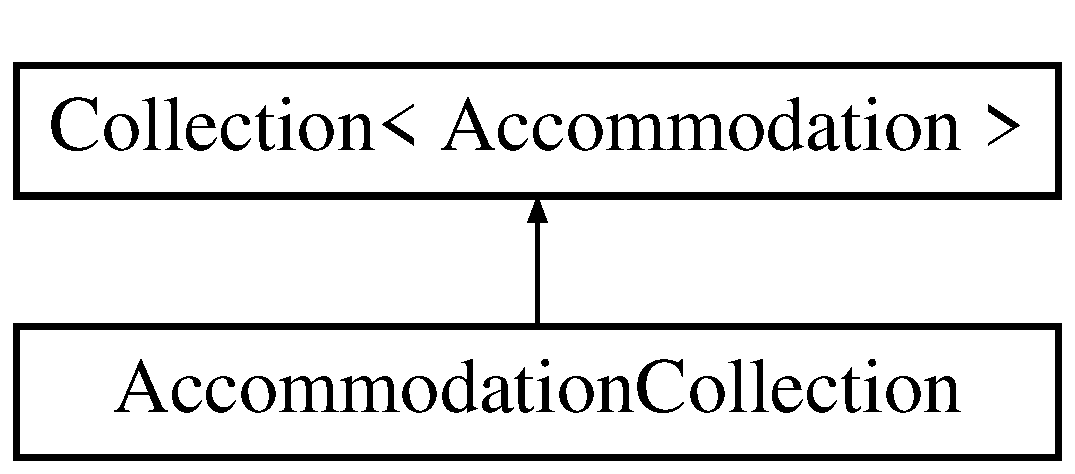
\includegraphics[height=2.000000cm]{class_accommodation_collection}
\end{center}
\end{figure}
\subsection*{Public Member Functions}
\begin{DoxyCompactItemize}
\item 
\mbox{\Hypertarget{class_accommodation_collection_accd0beebc1658e747c569a9d8c07bd1c}\label{class_accommodation_collection_accd0beebc1658e747c569a9d8c07bd1c}} 
void {\bfseries sortbycost} ()
\item 
\mbox{\Hypertarget{class_accommodation_collection_a9d5d3fe1e5c078e24553592a5d521178}\label{class_accommodation_collection_a9d5d3fe1e5c078e24553592a5d521178}} 
void {\bfseries sort\+By\+Date} ()
\end{DoxyCompactItemize}
\subsection*{Additional Inherited Members}


The documentation for this class was generated from the following files\+:\begin{DoxyCompactItemize}
\item 
src/Accommodation\+Collection.\+h\item 
src/Accommodation\+Collection.\+cpp\end{DoxyCompactItemize}

\hypertarget{classadd_accommodation}{}\section{add\+Accommodation Class Reference}
\label{classadd_accommodation}\index{add\+Accommodation@{add\+Accommodation}}


{\ttfamily \#include $<$add\+Accommodation.\+h$>$}

Inheritance diagram for add\+Accommodation\+:\begin{figure}[H]
\begin{center}
\leavevmode
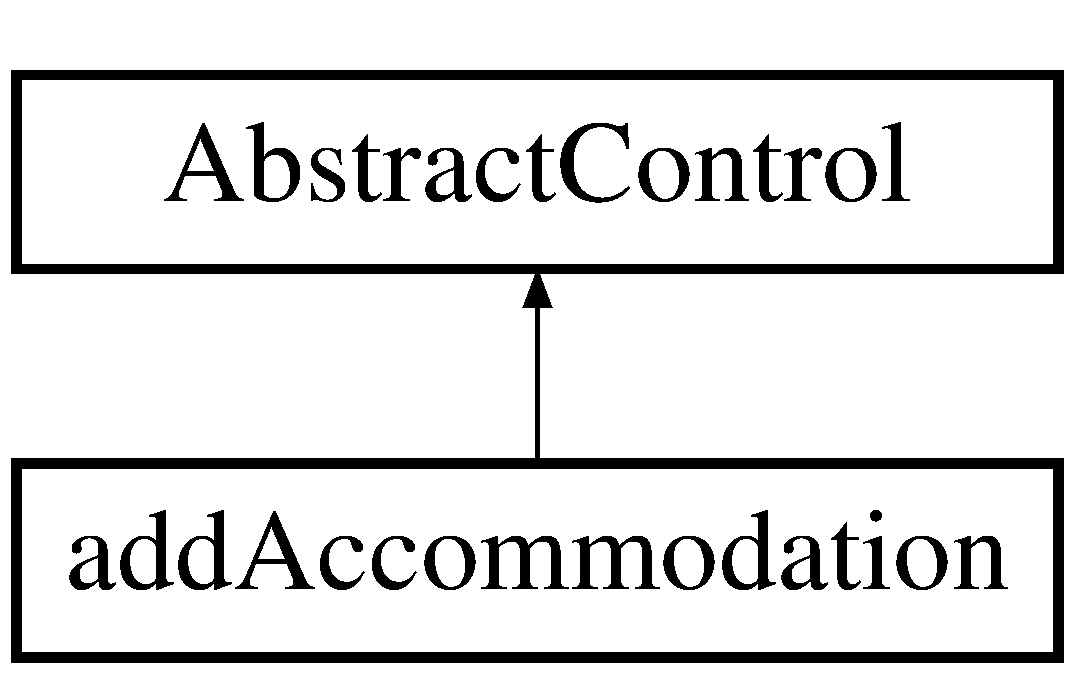
\includegraphics[height=2.000000cm]{classadd_accommodation}
\end{center}
\end{figure}
\subsection*{Public Member Functions}
\begin{DoxyCompactItemize}
\item 
\mbox{\Hypertarget{classadd_accommodation_a36fdd088c95c0af12d67bc678d346c78}\label{classadd_accommodation_a36fdd088c95c0af12d67bc678d346c78}} 
void {\bfseries add\+New\+Accommodation} (string hostid, string name, string address, int cost, string date, int opaque\+Cost)
\end{DoxyCompactItemize}
\subsection*{Additional Inherited Members}


\subsection{Detailed Description}
숙소 등록 Control 

The documentation for this class was generated from the following files\+:\begin{DoxyCompactItemize}
\item 
src/controls/add\+Accommodation.\+h\item 
src/controls/add\+Accommodation.\+cpp\end{DoxyCompactItemize}

\hypertarget{classadd_accommodation_u_i}{}\section{add\+Accommodation\+UI Class Reference}
\label{classadd_accommodation_u_i}\index{add\+Accommodation\+UI@{add\+Accommodation\+UI}}
Inheritance diagram for add\+Accommodation\+UI\+:\begin{figure}[H]
\begin{center}
\leavevmode
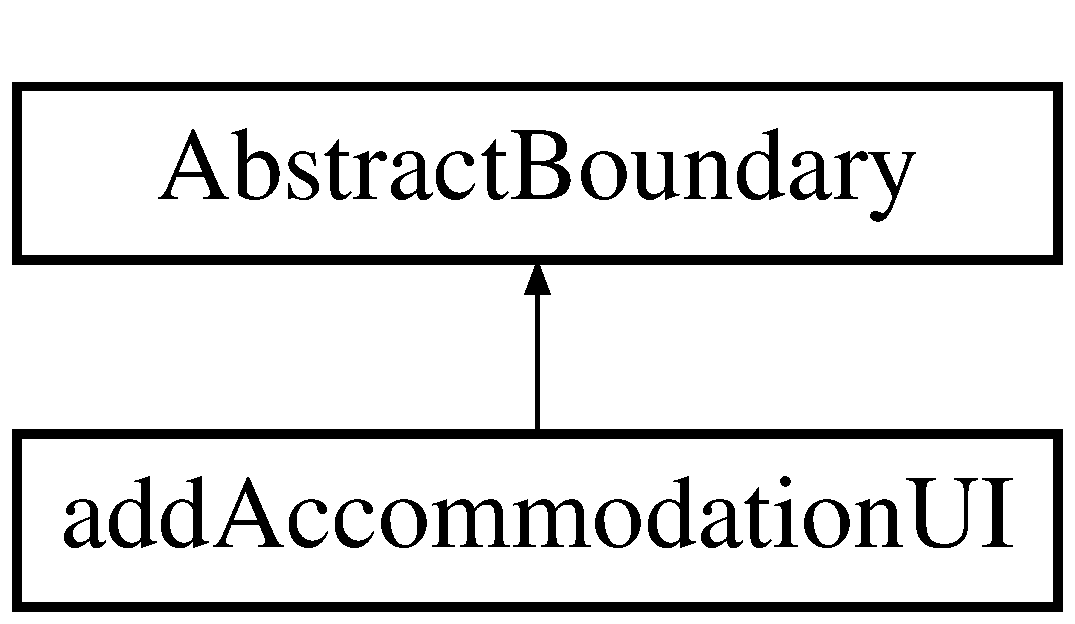
\includegraphics[height=2.000000cm]{classadd_accommodation_u_i}
\end{center}
\end{figure}
\subsection*{Public Member Functions}
\begin{DoxyCompactItemize}
\item 
\mbox{\Hypertarget{classadd_accommodation_u_i_aade79d966092990c38b6c23e447e2307}\label{classadd_accommodation_u_i_aade79d966092990c38b6c23e447e2307}} 
void {\bfseries create\+Accommodation} (string hostid, string name, string address, int cost, string date, int opaque\+Cost)
\end{DoxyCompactItemize}
\subsection*{Additional Inherited Members}


The documentation for this class was generated from the following files\+:\begin{DoxyCompactItemize}
\item 
src/boundaries/add\+Accommodation\+U\+I.\+h\item 
src/boundaries/add\+Accommodation\+U\+I.\+cpp\end{DoxyCompactItemize}

\hypertarget{class_collection}{}\section{Collection$<$ T $>$ Class Template Reference}
\label{class_collection}\index{Collection$<$ T $>$@{Collection$<$ T $>$}}
\subsection*{Public Member Functions}
\begin{DoxyCompactItemize}
\item 
T $\ast$ \mbox{\hyperlink{class_collection_a64cd1dc1f2099f0baa1e8ddb0efdd470}{get}} (int index)
\item 
void $\ast$ \mbox{\hyperlink{class_collection_ac05ab0d5f369c5a645123bad16d102c1}{add}} (T $\ast$)
\item 
int \mbox{\hyperlink{class_collection_a172de5b961f68075b07ce17c4dc79d94}{set}} (int index, T $\ast$item)
\item 
void \mbox{\hyperlink{class_collection_a11e03bd78c5b0234fe075b69f776b800}{remove}} (int index)
\item 
void \mbox{\hyperlink{class_collection_a6d5b06e5d2528c1251a5eb8b79ce756b}{remove}} (T $\ast$p\+Item)
\item 
int \mbox{\hyperlink{class_collection_a2fc76ab0d838768768ccb5df10aee711}{get\+Size}} ()
\item 
bool \mbox{\hyperlink{class_collection_a7c44d6d2aad8c98fbfe597646d7fd4ff}{exists}} (T $\ast$p\+Item)
\end{DoxyCompactItemize}
\subsection*{Protected Attributes}
\begin{DoxyCompactItemize}
\item 
\mbox{\Hypertarget{class_collection_a01e649ea61c423771fc84aed675996b4}\label{class_collection_a01e649ea61c423771fc84aed675996b4}} 
list$<$ T $\ast$ $>$ {\bfseries \+\_\+list}
\end{DoxyCompactItemize}


\subsection{Member Function Documentation}
\mbox{\Hypertarget{class_collection_ac05ab0d5f369c5a645123bad16d102c1}\label{class_collection_ac05ab0d5f369c5a645123bad16d102c1}} 
\index{Collection@{Collection}!add@{add}}
\index{add@{add}!Collection@{Collection}}
\subsubsection{\texorpdfstring{add()}{add()}}
{\footnotesize\ttfamily template$<$typename T$>$ \\
void $\ast$ \mbox{\hyperlink{class_collection}{Collection}}$<$ T $>$\+::add (\begin{DoxyParamCaption}\item[{T $\ast$}]{item }\end{DoxyParamCaption})}

collection에 item을 추가 \begin{DoxyReturn}{Returns}

\end{DoxyReturn}
\mbox{\Hypertarget{class_collection_a7c44d6d2aad8c98fbfe597646d7fd4ff}\label{class_collection_a7c44d6d2aad8c98fbfe597646d7fd4ff}} 
\index{Collection@{Collection}!exists@{exists}}
\index{exists@{exists}!Collection@{Collection}}
\subsubsection{\texorpdfstring{exists()}{exists()}}
{\footnotesize\ttfamily template$<$typename T$>$ \\
bool \mbox{\hyperlink{class_collection}{Collection}}$<$ T $>$\+::exists (\begin{DoxyParamCaption}\item[{T $\ast$}]{p\+Item }\end{DoxyParamCaption})}

collection에 Item 포함 여부 
\begin{DoxyParams}{Parameters}
{\em p\+Item} & \\
\hline
\end{DoxyParams}
\begin{DoxyReturn}{Returns}
포함 여부 
\end{DoxyReturn}
\mbox{\Hypertarget{class_collection_a64cd1dc1f2099f0baa1e8ddb0efdd470}\label{class_collection_a64cd1dc1f2099f0baa1e8ddb0efdd470}} 
\index{Collection@{Collection}!get@{get}}
\index{get@{get}!Collection@{Collection}}
\subsubsection{\texorpdfstring{get()}{get()}}
{\footnotesize\ttfamily template$<$typename T $>$ \\
T $\ast$ \mbox{\hyperlink{class_collection}{Collection}}$<$ T $>$\+::get (\begin{DoxyParamCaption}\item[{int}]{index }\end{DoxyParamCaption})}

해당 index의 item를 반환 
\begin{DoxyParams}{Parameters}
{\em index} & \\
\hline
\end{DoxyParams}
\begin{DoxyReturn}{Returns}
item 
\end{DoxyReturn}
\mbox{\Hypertarget{class_collection_a2fc76ab0d838768768ccb5df10aee711}\label{class_collection_a2fc76ab0d838768768ccb5df10aee711}} 
\index{Collection@{Collection}!get\+Size@{get\+Size}}
\index{get\+Size@{get\+Size}!Collection@{Collection}}
\subsubsection{\texorpdfstring{get\+Size()}{getSize()}}
{\footnotesize\ttfamily template$<$typename T $>$ \\
int \mbox{\hyperlink{class_collection}{Collection}}$<$ T $>$\+::get\+Size (\begin{DoxyParamCaption}{ }\end{DoxyParamCaption})}

collection의 item 갯수 반환 \begin{DoxyReturn}{Returns}
item 갯수 
\end{DoxyReturn}
\mbox{\Hypertarget{class_collection_a11e03bd78c5b0234fe075b69f776b800}\label{class_collection_a11e03bd78c5b0234fe075b69f776b800}} 
\index{Collection@{Collection}!remove@{remove}}
\index{remove@{remove}!Collection@{Collection}}
\subsubsection{\texorpdfstring{remove()}{remove()}\hspace{0.1cm}{\footnotesize\ttfamily [1/2]}}
{\footnotesize\ttfamily template$<$typename T $>$ \\
void \mbox{\hyperlink{class_collection}{Collection}}$<$ T $>$\+::remove (\begin{DoxyParamCaption}\item[{int}]{index }\end{DoxyParamCaption})}

해당 index의 item을 collection에서 삭제 
\begin{DoxyParams}{Parameters}
{\em 성공} & 여부 \\
\hline
\end{DoxyParams}
\mbox{\Hypertarget{class_collection_a6d5b06e5d2528c1251a5eb8b79ce756b}\label{class_collection_a6d5b06e5d2528c1251a5eb8b79ce756b}} 
\index{Collection@{Collection}!remove@{remove}}
\index{remove@{remove}!Collection@{Collection}}
\subsubsection{\texorpdfstring{remove()}{remove()}\hspace{0.1cm}{\footnotesize\ttfamily [2/2]}}
{\footnotesize\ttfamily template$<$typename T$>$ \\
void \mbox{\hyperlink{class_collection}{Collection}}$<$ T $>$\+::remove (\begin{DoxyParamCaption}\item[{T $\ast$}]{p\+Item }\end{DoxyParamCaption})}

해당 item을 collection에서 삭제 
\begin{DoxyParams}{Parameters}
{\em p\+Item} & \\
\hline
\end{DoxyParams}
\mbox{\Hypertarget{class_collection_a172de5b961f68075b07ce17c4dc79d94}\label{class_collection_a172de5b961f68075b07ce17c4dc79d94}} 
\index{Collection@{Collection}!set@{set}}
\index{set@{set}!Collection@{Collection}}
\subsubsection{\texorpdfstring{set()}{set()}}
{\footnotesize\ttfamily template$<$typename T$>$ \\
int \mbox{\hyperlink{class_collection}{Collection}}$<$ T $>$\+::set (\begin{DoxyParamCaption}\item[{int}]{index,  }\item[{T $\ast$}]{item }\end{DoxyParamCaption})}

해당 index에 새로운 멤버 삽입 또는 교체 
\begin{DoxyParams}{Parameters}
{\em index} & \\
\hline
\end{DoxyParams}


The documentation for this class was generated from the following file\+:\begin{DoxyCompactItemize}
\item 
src/Collection.\+h\end{DoxyCompactItemize}

\hypertarget{class_date_time_utils}{}\section{Date\+Time\+Utils Class Reference}
\label{class_date_time_utils}\index{Date\+Time\+Utils@{Date\+Time\+Utils}}
\subsection*{Static Public Member Functions}
\begin{DoxyCompactItemize}
\item 
\mbox{\Hypertarget{class_date_time_utils_a0116f7ee9d799e4a4a52975c79600a65}\label{class_date_time_utils_a0116f7ee9d799e4a4a52975c79600a65}} 
static string {\bfseries add\+Days} (string time, int days)
\item 
\mbox{\Hypertarget{class_date_time_utils_aee21079e4db5bca85131a7c70c5475e1}\label{class_date_time_utils_aee21079e4db5bca85131a7c70c5475e1}} 
static string {\bfseries add\+Years} (string time, int years)
\end{DoxyCompactItemize}


The documentation for this class was generated from the following files\+:\begin{DoxyCompactItemize}
\item 
src/Date\+Time\+Utils.\+h\item 
src/Date\+Time\+Utils.\+cpp\end{DoxyCompactItemize}

\hypertarget{class_guest}{}\section{Guest Class Reference}
\label{class_guest}\index{Guest@{Guest}}
Inheritance diagram for Guest\+:\begin{figure}[H]
\begin{center}
\leavevmode
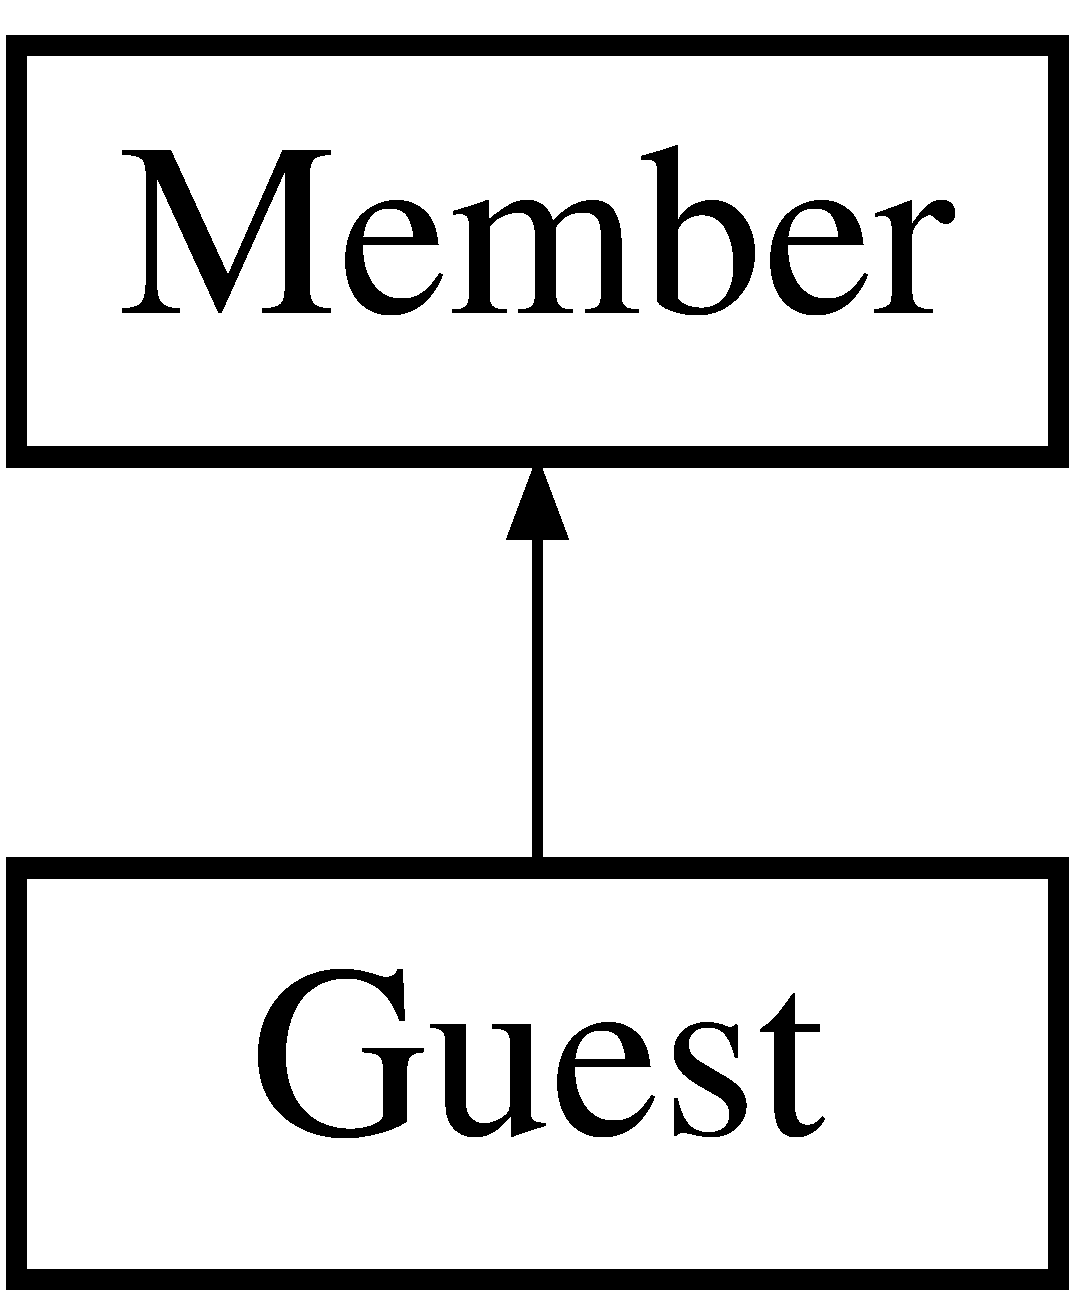
\includegraphics[height=2.000000cm]{class_guest}
\end{center}
\end{figure}
\subsection*{Public Member Functions}
\begin{DoxyCompactItemize}
\item 
\mbox{\Hypertarget{class_guest_a16883a872c23d3b57c330a8c18031795}\label{class_guest_a16883a872c23d3b57c330a8c18031795}} 
{\bfseries Guest} (const string \&name, const string \&security\+Number, const string \&address, const string \&id, const string \&password)
\item 
\mbox{\Hypertarget{class_guest_a9d8fc5c2d74eb419edb0c0ad1f16a73e}\label{class_guest_a9d8fc5c2d74eb419edb0c0ad1f16a73e}} 
const string {\bfseries get\+Last\+Opaque\+Try\+Time} () const
\item 
\mbox{\Hypertarget{class_guest_a89ceffdfdbf729a0e2ae3592459fcae6}\label{class_guest_a89ceffdfdbf729a0e2ae3592459fcae6}} 
void {\bfseries set\+Last\+Opaque\+Try\+Time} (const string \&last\+Opaque\+Try\+Time)
\end{DoxyCompactItemize}


The documentation for this class was generated from the following files\+:\begin{DoxyCompactItemize}
\item 
src/Guest.\+h\item 
src/Guest.\+cpp\end{DoxyCompactItemize}

\hypertarget{class_host}{}\section{Host Class Reference}
\label{class_host}\index{Host@{Host}}
Inheritance diagram for Host\+:\begin{figure}[H]
\begin{center}
\leavevmode
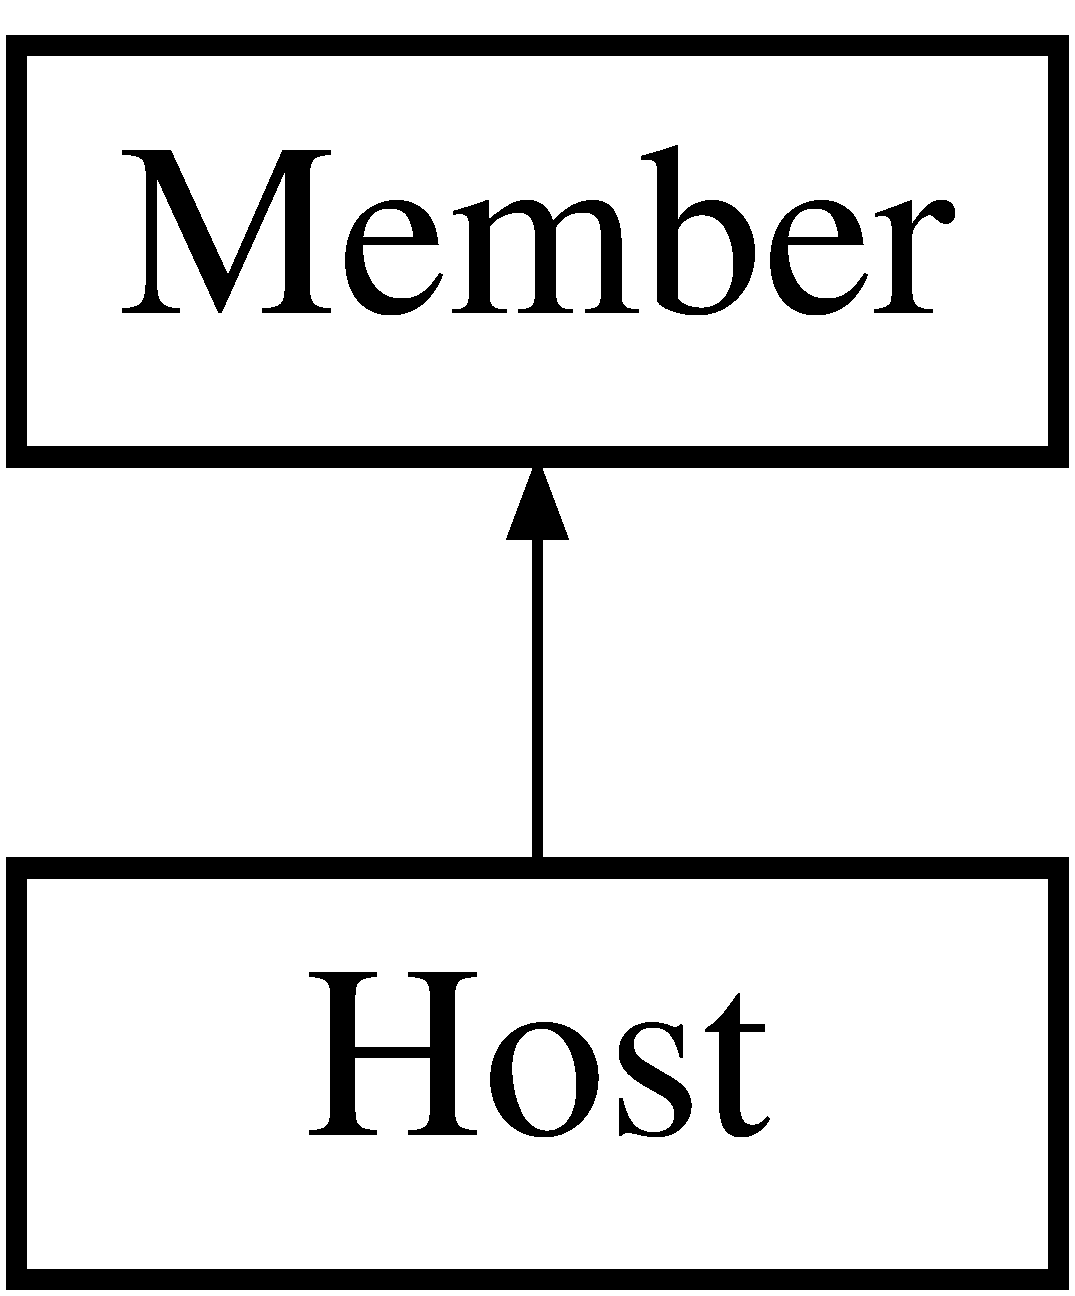
\includegraphics[height=2.000000cm]{class_host}
\end{center}
\end{figure}
\subsection*{Public Member Functions}
\begin{DoxyCompactItemize}
\item 
\mbox{\Hypertarget{class_host_a9f21538946cb995974ab3512de663ccd}\label{class_host_a9f21538946cb995974ab3512de663ccd}} 
{\bfseries Host} (const string \&name, const string \&security\+Number, const string \&address, const string \&id, const string \&password)
\item 
\mbox{\Hypertarget{class_host_a6c9ac82f8263c26b0382ae6b3b52b82d}\label{class_host_a6c9ac82f8263c26b0382ae6b3b52b82d}} 
\mbox{\hyperlink{class_accommodation_collection}{Accommodation\+Collection}} $\ast$ {\bfseries get\+Accommodations} ()
\end{DoxyCompactItemize}


The documentation for this class was generated from the following files\+:\begin{DoxyCompactItemize}
\item 
src/Host.\+h\item 
src/Host.\+cpp\end{DoxyCompactItemize}

\hypertarget{class_list_host_accommodation_control}{}\section{List\+Host\+Accommodation\+Control Class Reference}
\label{class_list_host_accommodation_control}\index{List\+Host\+Accommodation\+Control@{List\+Host\+Accommodation\+Control}}
Inheritance diagram for List\+Host\+Accommodation\+Control\+:\begin{figure}[H]
\begin{center}
\leavevmode
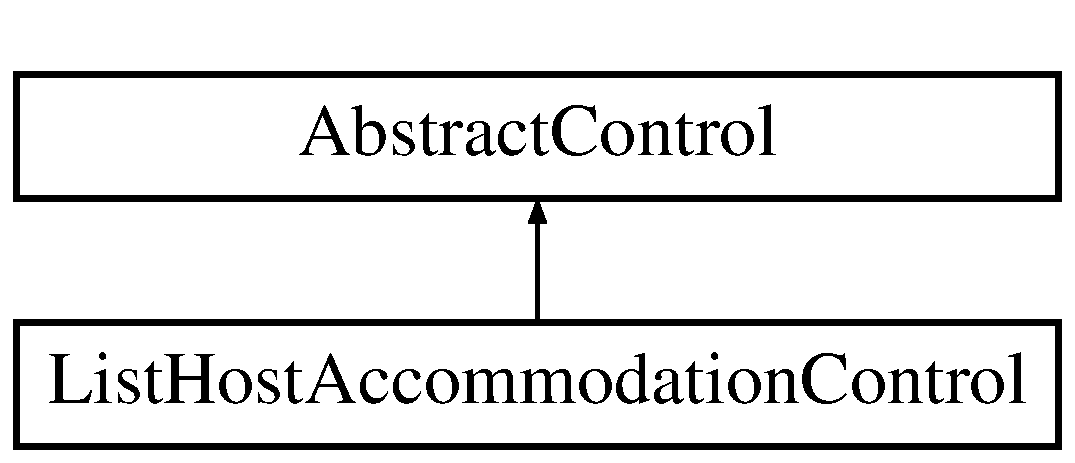
\includegraphics[height=2.000000cm]{class_list_host_accommodation_control}
\end{center}
\end{figure}
\subsection*{Public Member Functions}
\begin{DoxyCompactItemize}
\item 
\mbox{\Hypertarget{class_list_host_accommodation_control_a81b570b7ff3da104613be89c3899db39}\label{class_list_host_accommodation_control_a81b570b7ff3da104613be89c3899db39}} 
void {\bfseries list\+Accommodations} ()
\end{DoxyCompactItemize}
\subsection*{Additional Inherited Members}


The documentation for this class was generated from the following files\+:\begin{DoxyCompactItemize}
\item 
src/controls/List\+Host\+Accommodation\+Control.\+h\item 
src/controls/List\+Host\+Accommodation\+Control.\+cpp\end{DoxyCompactItemize}

\hypertarget{class_list_host_accommodation_u_i}{}\section{List\+Host\+Accommodation\+UI Class Reference}
\label{class_list_host_accommodation_u_i}\index{List\+Host\+Accommodation\+UI@{List\+Host\+Accommodation\+UI}}
Inheritance diagram for List\+Host\+Accommodation\+UI\+:\begin{figure}[H]
\begin{center}
\leavevmode
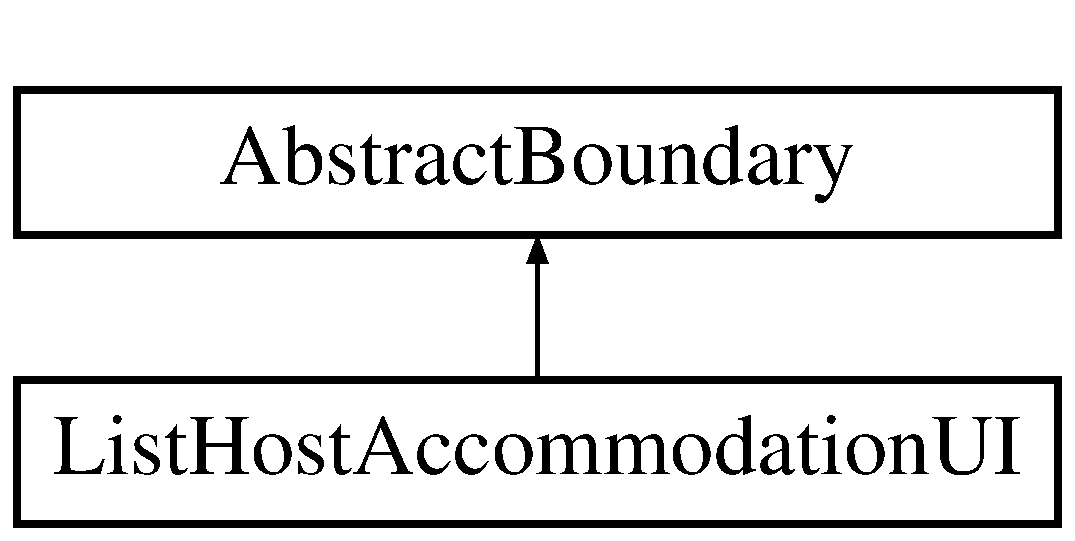
\includegraphics[height=2.000000cm]{class_list_host_accommodation_u_i}
\end{center}
\end{figure}
\subsection*{Public Member Functions}
\begin{DoxyCompactItemize}
\item 
\mbox{\Hypertarget{class_list_host_accommodation_u_i_a757ecf0a13adf19cdb60b581a59605bc}\label{class_list_host_accommodation_u_i_a757ecf0a13adf19cdb60b581a59605bc}} 
void {\bfseries on\+List\+Accommodation} ()
\end{DoxyCompactItemize}
\subsection*{Additional Inherited Members}


The documentation for this class was generated from the following files\+:\begin{DoxyCompactItemize}
\item 
src/boundaries/List\+Host\+Accommodation\+U\+I.\+h\item 
src/boundaries/List\+Host\+Accommodation\+U\+I.\+cpp\end{DoxyCompactItemize}

\hypertarget{class_login_control}{}\section{Login\+Control Class Reference}
\label{class_login_control}\index{Login\+Control@{Login\+Control}}


{\ttfamily \#include $<$Login\+Control.\+h$>$}

Inheritance diagram for Login\+Control\+:\begin{figure}[H]
\begin{center}
\leavevmode
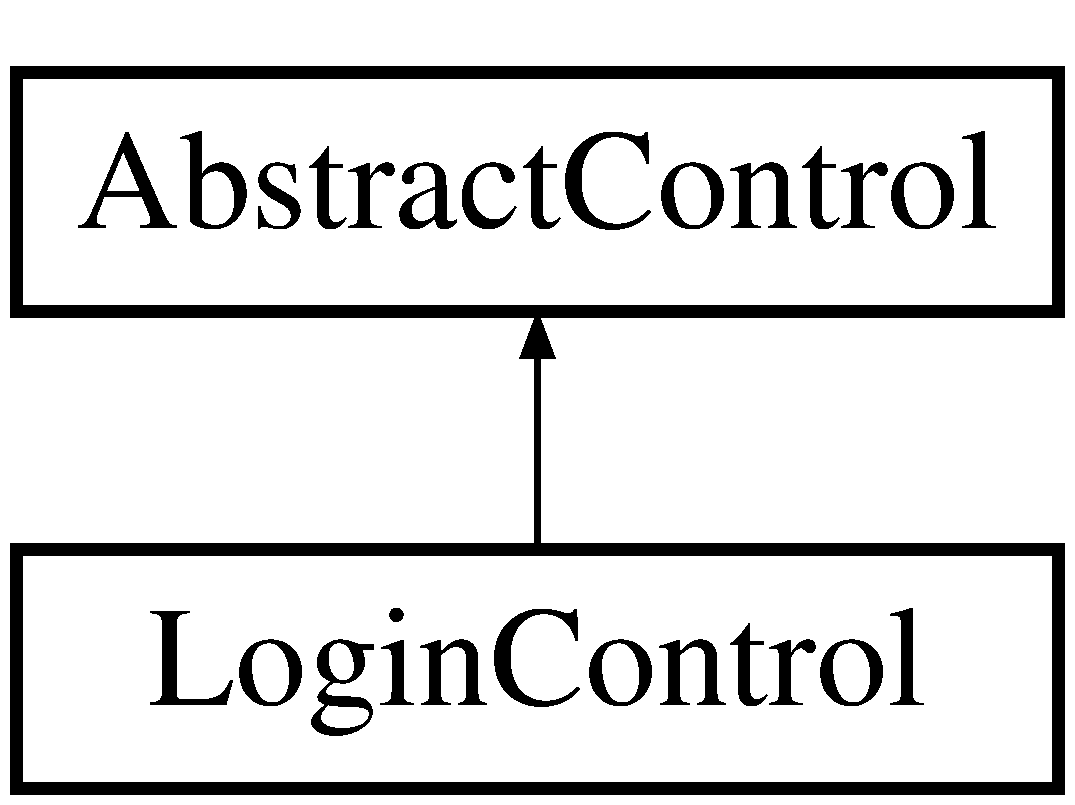
\includegraphics[height=2.000000cm]{class_login_control}
\end{center}
\end{figure}
\subsection*{Public Member Functions}
\begin{DoxyCompactItemize}
\item 
void \mbox{\hyperlink{class_login_control_aff5b73021c402918a3e6de18b326367f}{try\+Login}} (string id, string password)
\end{DoxyCompactItemize}
\subsection*{Additional Inherited Members}


\subsection{Detailed Description}
로그인 관련 Control 

\subsection{Member Function Documentation}
\mbox{\Hypertarget{class_login_control_aff5b73021c402918a3e6de18b326367f}\label{class_login_control_aff5b73021c402918a3e6de18b326367f}} 
\index{Login\+Control@{Login\+Control}!try\+Login@{try\+Login}}
\index{try\+Login@{try\+Login}!Login\+Control@{Login\+Control}}
\subsubsection{\texorpdfstring{try\+Login()}{tryLogin()}}
{\footnotesize\ttfamily void Login\+Control\+::try\+Login (\begin{DoxyParamCaption}\item[{string}]{id,  }\item[{string}]{password }\end{DoxyParamCaption})}

Login을 시도 
\begin{DoxyParams}{Parameters}
{\em id} & \\
\hline
{\em password} & \\
\hline
\end{DoxyParams}


The documentation for this class was generated from the following files\+:\begin{DoxyCompactItemize}
\item 
src/controls/Login\+Control.\+h\item 
src/controls/Login\+Control.\+cpp\end{DoxyCompactItemize}

\hypertarget{class_login_u_i}{}\section{Login\+UI Class Reference}
\label{class_login_u_i}\index{Login\+UI@{Login\+UI}}
Inheritance diagram for Login\+UI\+:\begin{figure}[H]
\begin{center}
\leavevmode
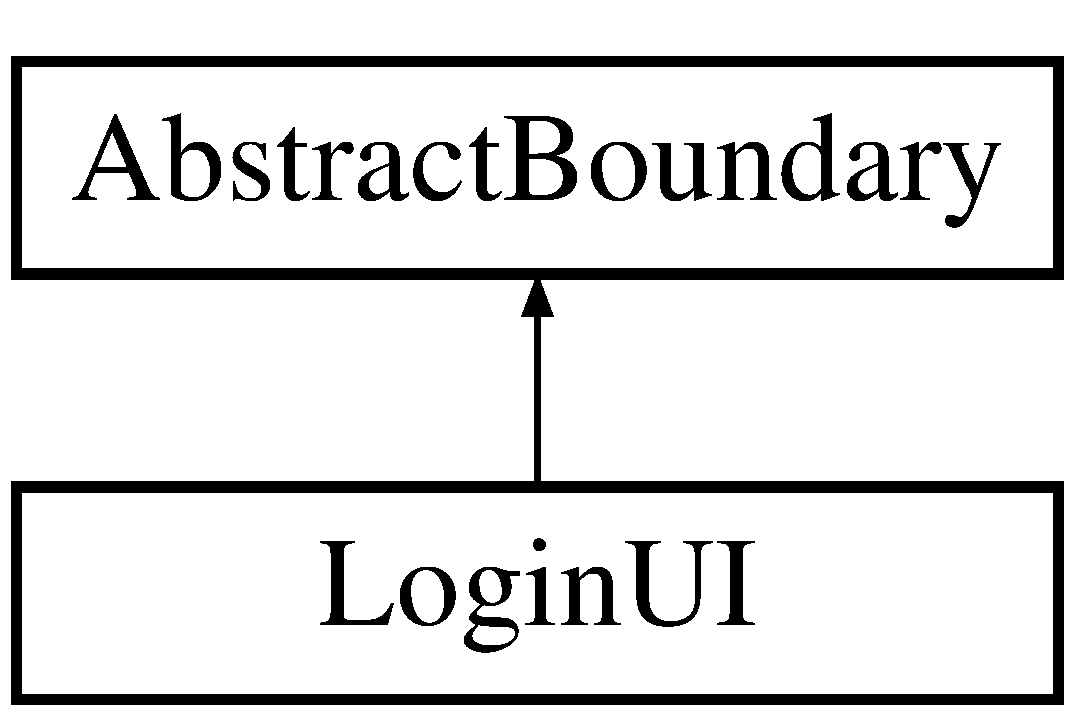
\includegraphics[height=2.000000cm]{class_login_u_i}
\end{center}
\end{figure}
\subsection*{Public Member Functions}
\begin{DoxyCompactItemize}
\item 
\mbox{\Hypertarget{class_login_u_i_a5f384aaed36f6ee7c7f78d4a905cd77f}\label{class_login_u_i_a5f384aaed36f6ee7c7f78d4a905cd77f}} 
void {\bfseries on\+Request\+Login} (string id, string password)
\end{DoxyCompactItemize}
\subsection*{Additional Inherited Members}


The documentation for this class was generated from the following files\+:\begin{DoxyCompactItemize}
\item 
src/boundaries/Login\+U\+I.\+h\item 
src/boundaries/Login\+U\+I.\+cpp\end{DoxyCompactItemize}

\hypertarget{class_logout_control}{}\section{Logout\+Control Class Reference}
\label{class_logout_control}\index{Logout\+Control@{Logout\+Control}}


{\ttfamily \#include $<$Logout\+Control.\+h$>$}

Inheritance diagram for Logout\+Control\+:\begin{figure}[H]
\begin{center}
\leavevmode
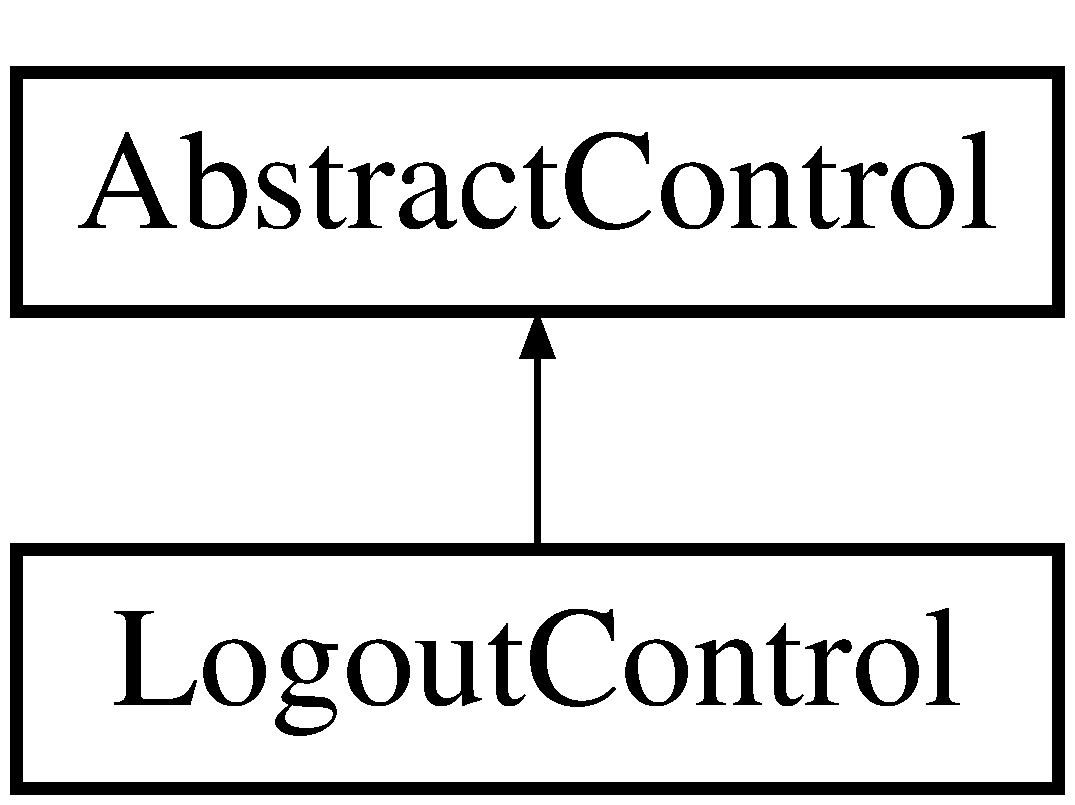
\includegraphics[height=2.000000cm]{class_logout_control}
\end{center}
\end{figure}
\subsection*{Public Member Functions}
\begin{DoxyCompactItemize}
\item 
void \mbox{\hyperlink{class_logout_control_a312833da79ce891bcfd9879f8a5a2d52}{try\+Logout}} ()
\end{DoxyCompactItemize}
\subsection*{Additional Inherited Members}


\subsection{Detailed Description}
로그아웃 Control 

\subsection{Member Function Documentation}
\mbox{\Hypertarget{class_logout_control_a312833da79ce891bcfd9879f8a5a2d52}\label{class_logout_control_a312833da79ce891bcfd9879f8a5a2d52}} 
\index{Logout\+Control@{Logout\+Control}!try\+Logout@{try\+Logout}}
\index{try\+Logout@{try\+Logout}!Logout\+Control@{Logout\+Control}}
\subsubsection{\texorpdfstring{try\+Logout()}{tryLogout()}}
{\footnotesize\ttfamily void Logout\+Control\+::try\+Logout (\begin{DoxyParamCaption}{ }\end{DoxyParamCaption})}

로그아웃을 시도함 

The documentation for this class was generated from the following files\+:\begin{DoxyCompactItemize}
\item 
src/controls/Logout\+Control.\+h\item 
src/controls/Logout\+Control.\+cpp\end{DoxyCompactItemize}

\hypertarget{class_logout_u_i}{}\section{Logout\+UI Class Reference}
\label{class_logout_u_i}\index{Logout\+UI@{Logout\+UI}}
Inheritance diagram for Logout\+UI\+:\begin{figure}[H]
\begin{center}
\leavevmode
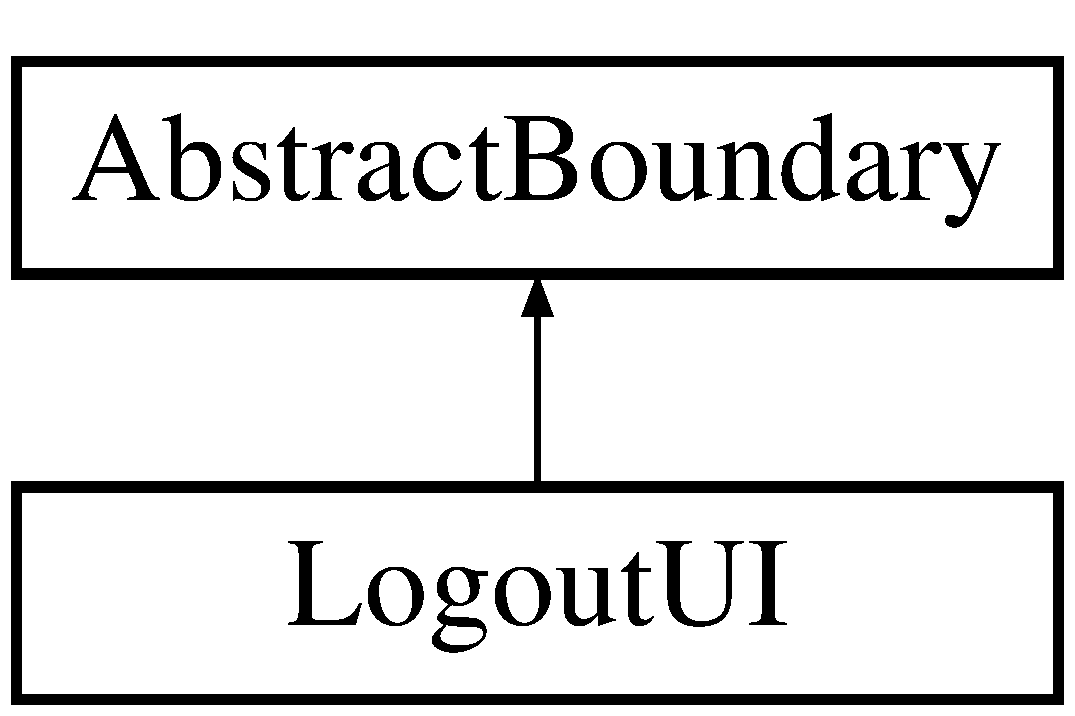
\includegraphics[height=2.000000cm]{class_logout_u_i}
\end{center}
\end{figure}
\subsection*{Public Member Functions}
\begin{DoxyCompactItemize}
\item 
\mbox{\Hypertarget{class_logout_u_i_a02c30caf68fb9a3fd9b094b19c18af81}\label{class_logout_u_i_a02c30caf68fb9a3fd9b094b19c18af81}} 
void {\bfseries on\+Request\+Logout} ()
\end{DoxyCompactItemize}
\subsection*{Additional Inherited Members}


The documentation for this class was generated from the following files\+:\begin{DoxyCompactItemize}
\item 
src/boundaries/Logout\+U\+I.\+h\item 
src/boundaries/Logout\+U\+I.\+cpp\end{DoxyCompactItemize}

\hypertarget{class_member}{}\section{Member Class Reference}
\label{class_member}\index{Member@{Member}}


{\ttfamily \#include $<$Member.\+h$>$}

Inheritance diagram for Member\+:\begin{figure}[H]
\begin{center}
\leavevmode
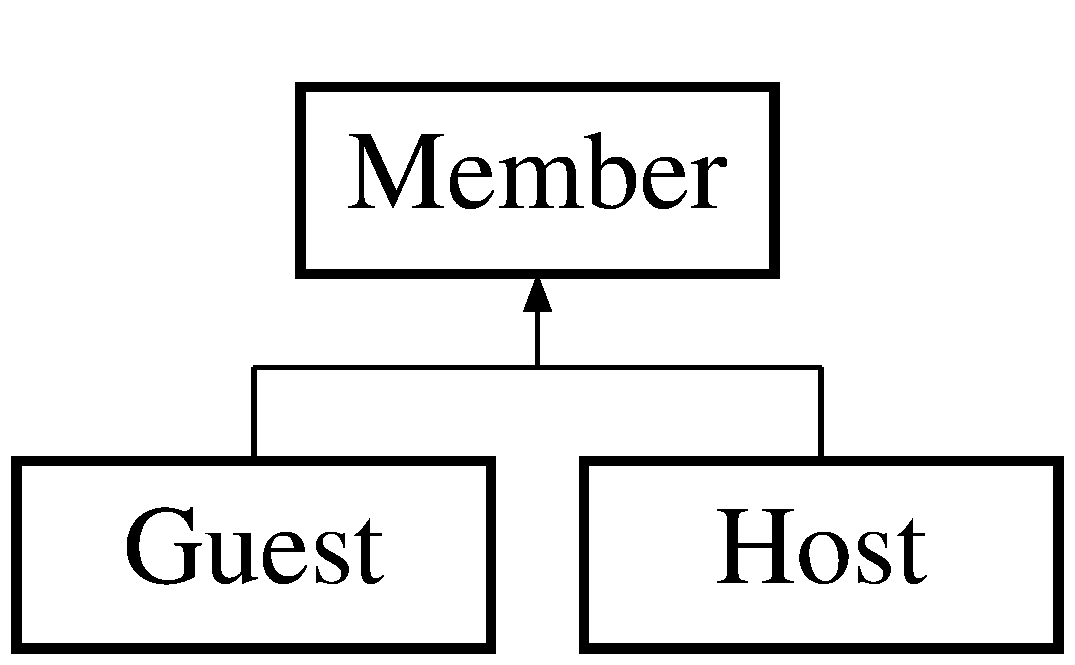
\includegraphics[height=2.000000cm]{class_member}
\end{center}
\end{figure}
\subsection*{Public Member Functions}
\begin{DoxyCompactItemize}
\item 
\mbox{\Hypertarget{class_member_af48adfcb614a6e5501237dc93e07ab2c}\label{class_member_af48adfcb614a6e5501237dc93e07ab2c}} 
{\bfseries Member} (Member\+Types type, string name, string security\+Number, string address, string id, string password)
\item 
\mbox{\Hypertarget{class_member_accf776380b3a2f391b4f57e1d938a071}\label{class_member_accf776380b3a2f391b4f57e1d938a071}} 
Member\+Types {\bfseries get\+Type} ()
\item 
\mbox{\Hypertarget{class_member_acbe6a0cd073a21fb0f1da2cbfb260952}\label{class_member_acbe6a0cd073a21fb0f1da2cbfb260952}} 
string {\bfseries get\+Name} ()
\item 
\mbox{\Hypertarget{class_member_a737850218112eb82ae1d81789c1244e1}\label{class_member_a737850218112eb82ae1d81789c1244e1}} 
string {\bfseries get\+Address} ()
\item 
\mbox{\Hypertarget{class_member_ae486cfbc7e5ab2fc5705115c4f96b2c2}\label{class_member_ae486cfbc7e5ab2fc5705115c4f96b2c2}} 
string {\bfseries get\+ID} ()
\item 
bool \mbox{\hyperlink{class_member_a9fe3103fb15b00e6a51194d57f6c4148}{equals\+Password}} (string password)
\end{DoxyCompactItemize}


\subsection{Detailed Description}
회원 정보에 관한 Class 

\subsection{Member Function Documentation}
\mbox{\Hypertarget{class_member_a9fe3103fb15b00e6a51194d57f6c4148}\label{class_member_a9fe3103fb15b00e6a51194d57f6c4148}} 
\index{Member@{Member}!equals\+Password@{equals\+Password}}
\index{equals\+Password@{equals\+Password}!Member@{Member}}
\subsubsection{\texorpdfstring{equals\+Password()}{equalsPassword()}}
{\footnotesize\ttfamily bool Member\+::equals\+Password (\begin{DoxyParamCaption}\item[{string}]{password }\end{DoxyParamCaption})}

패스워드 일치 여부 체크 
\begin{DoxyParams}{Parameters}
{\em password} & \\
\hline
\end{DoxyParams}
\begin{DoxyReturn}{Returns}
일치 여부 
\end{DoxyReturn}


The documentation for this class was generated from the following files\+:\begin{DoxyCompactItemize}
\item 
src/Member.\+h\item 
src/Member.\+cpp\end{DoxyCompactItemize}

\hypertarget{class_member_collection}{}\section{Member\+Collection Class Reference}
\label{class_member_collection}\index{Member\+Collection@{Member\+Collection}}
Inheritance diagram for Member\+Collection\+:\begin{figure}[H]
\begin{center}
\leavevmode
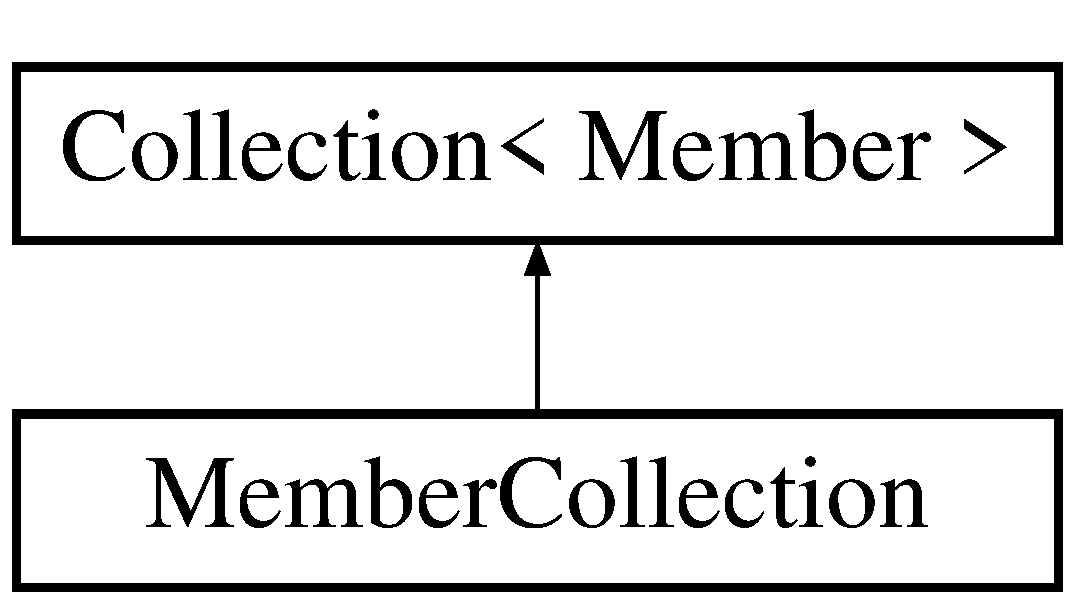
\includegraphics[height=2.000000cm]{class_member_collection}
\end{center}
\end{figure}
\subsection*{Additional Inherited Members}


The documentation for this class was generated from the following files\+:\begin{DoxyCompactItemize}
\item 
src/Member\+Collection.\+h\item 
src/Member\+Collection.\+cpp\end{DoxyCompactItemize}

\hypertarget{class_opaque}{}\section{Opaque Class Reference}
\label{class_opaque}\index{Opaque@{Opaque}}


The documentation for this class was generated from the following file\+:\begin{DoxyCompactItemize}
\item 
src/Opaque.\+h\end{DoxyCompactItemize}

\hypertarget{class_opaque_inventory_control}{}\section{Opaque\+Inventory\+Control Class Reference}
\label{class_opaque_inventory_control}\index{Opaque\+Inventory\+Control@{Opaque\+Inventory\+Control}}


{\ttfamily \#include $<$Opaque\+Inventory\+Control.\+h$>$}

Inheritance diagram for Opaque\+Inventory\+Control\+:\begin{figure}[H]
\begin{center}
\leavevmode
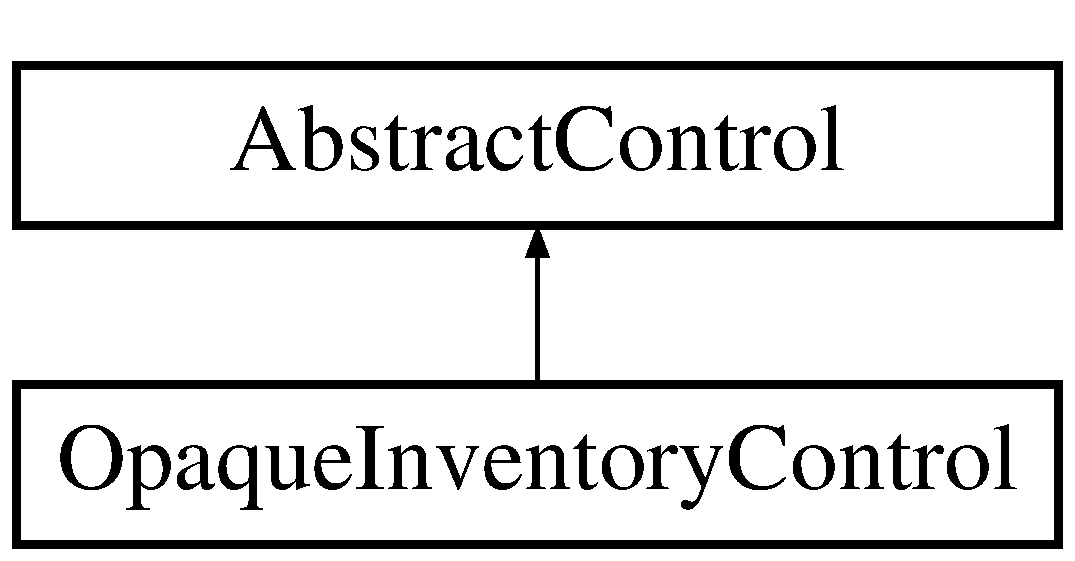
\includegraphics[height=2.000000cm]{class_opaque_inventory_control}
\end{center}
\end{figure}
\subsection*{Public Member Functions}
\begin{DoxyCompactItemize}
\item 
void \mbox{\hyperlink{class_opaque_inventory_control_a671ed0b02c98801a5f568a710b8fc107}{try\+Opaque\+Inventory\+Reservation}} (string address, string date, int opaque\+Cost)
\item 
\mbox{\Hypertarget{class_opaque_inventory_control_ab3db8bcd22d72ee5d34d7d435b6776ca}\label{class_opaque_inventory_control_ab3db8bcd22d72ee5d34d7d435b6776ca}} 
string {\bfseries add\+Opaque\+Reservation} (string hostid, string accommodation, int opaque\+Cost)
\end{DoxyCompactItemize}
\subsection*{Additional Inherited Members}


\subsection{Detailed Description}
Opaque\+Inventory 예약 시도 Control 

\subsection{Member Function Documentation}
\mbox{\Hypertarget{class_opaque_inventory_control_a671ed0b02c98801a5f568a710b8fc107}\label{class_opaque_inventory_control_a671ed0b02c98801a5f568a710b8fc107}} 
\index{Opaque\+Inventory\+Control@{Opaque\+Inventory\+Control}!try\+Opaque\+Inventory\+Reservation@{try\+Opaque\+Inventory\+Reservation}}
\index{try\+Opaque\+Inventory\+Reservation@{try\+Opaque\+Inventory\+Reservation}!Opaque\+Inventory\+Control@{Opaque\+Inventory\+Control}}
\subsubsection{\texorpdfstring{try\+Opaque\+Inventory\+Reservation()}{tryOpaqueInventoryReservation()}}
{\footnotesize\ttfamily void Opaque\+Inventory\+Control\+::try\+Opaque\+Inventory\+Reservation (\begin{DoxyParamCaption}\item[{string}]{address,  }\item[{string}]{date,  }\item[{int}]{opaque\+Cost }\end{DoxyParamCaption})}

Opaque\+Inventory 예약을 시도 
\begin{DoxyParams}{Parameters}
{\em address} & \\
\hline
{\em date} & \\
\hline
{\em opaque\+Cost} & \\
\hline
\end{DoxyParams}


The documentation for this class was generated from the following files\+:\begin{DoxyCompactItemize}
\item 
src/controls/Opaque\+Inventory\+Control.\+h\item 
src/controls/Opaque\+Inventory\+Control.\+cpp\end{DoxyCompactItemize}

\hypertarget{class_opaque_inventory_u_i}{}\section{Opaque\+Inventory\+UI Class Reference}
\label{class_opaque_inventory_u_i}\index{Opaque\+Inventory\+UI@{Opaque\+Inventory\+UI}}
Inheritance diagram for Opaque\+Inventory\+UI\+:\begin{figure}[H]
\begin{center}
\leavevmode
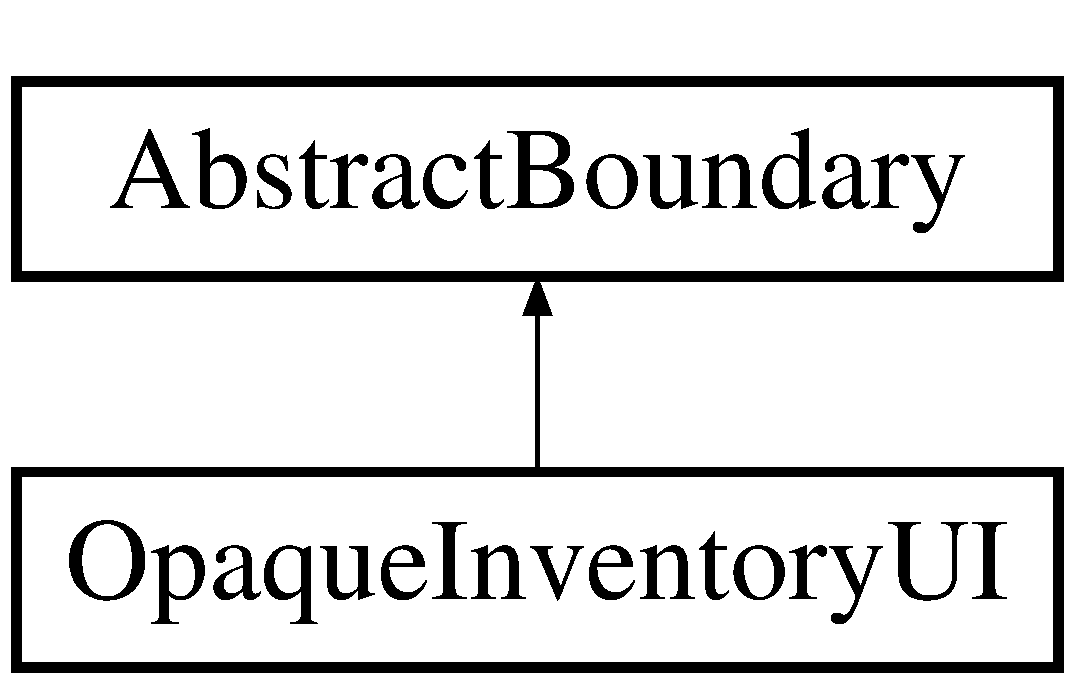
\includegraphics[height=2.000000cm]{class_opaque_inventory_u_i}
\end{center}
\end{figure}
\subsection*{Public Member Functions}
\begin{DoxyCompactItemize}
\item 
\mbox{\Hypertarget{class_opaque_inventory_u_i_afa5550666cb6f3616f6a23e738e049c8}\label{class_opaque_inventory_u_i_afa5550666cb6f3616f6a23e738e049c8}} 
void {\bfseries on\+Opaque\+Reservation\+Request} (string address, string date, int opaque\+Cost)
\end{DoxyCompactItemize}
\subsection*{Additional Inherited Members}


The documentation for this class was generated from the following files\+:\begin{DoxyCompactItemize}
\item 
src/boundaries/Opaque\+Inventory\+U\+I.\+h\item 
src/boundaries/Opaque\+Inventory\+U\+I.\+cpp\end{DoxyCompactItemize}

\hypertarget{class_output_writer}{}\section{Output\+Writer Class Reference}
\label{class_output_writer}\index{Output\+Writer@{Output\+Writer}}


{\ttfamily \#include $<$Output\+Writer.\+h$>$}

\subsection*{Public Member Functions}
\begin{DoxyCompactItemize}
\item 
\mbox{\Hypertarget{class_output_writer_a33a96359971dfce8fafdebac909bdd08}\label{class_output_writer_a33a96359971dfce8fafdebac909bdd08}} 
void {\bfseries open} (string file\+Name)
\item 
\mbox{\Hypertarget{class_output_writer_ab802980c4b874cb35ae744a170b5fd89}\label{class_output_writer_ab802980c4b874cb35ae744a170b5fd89}} 
void {\bfseries close} ()
\item 
\mbox{\Hypertarget{class_output_writer_a6f4f8d99eca724f6fcbb60bcb950a4e9}\label{class_output_writer_a6f4f8d99eca724f6fcbb60bcb950a4e9}} 
void {\bfseries write} (string fmt,...)
\item 
\mbox{\Hypertarget{class_output_writer_a17a9fd09b2241b8440ba24057e97e621}\label{class_output_writer_a17a9fd09b2241b8440ba24057e97e621}} 
void {\bfseries write\+Line} (string fmt,...)
\item 
\mbox{\Hypertarget{class_output_writer_a6affce047db6e83ac534488e90462047}\label{class_output_writer_a6affce047db6e83ac534488e90462047}} 
void {\bfseries write\+Line} ()
\end{DoxyCompactItemize}
\subsection*{Friends}
\begin{DoxyCompactItemize}
\item 
\mbox{\Hypertarget{class_output_writer_a184f0c3382d2d98357915f83d1d821c6}\label{class_output_writer_a184f0c3382d2d98357915f83d1d821c6}} 
class {\bfseries Abstract\+Boundary}
\end{DoxyCompactItemize}


\subsection{Detailed Description}
File Writing 과 관련된 Class 

The documentation for this class was generated from the following files\+:\begin{DoxyCompactItemize}
\item 
src/Output\+Writer.\+h\item 
src/Output\+Writer.\+cpp\end{DoxyCompactItemize}

\hypertarget{class_register_control}{}\section{Register\+Control Class Reference}
\label{class_register_control}\index{Register\+Control@{Register\+Control}}
Inheritance diagram for Register\+Control\+:\begin{figure}[H]
\begin{center}
\leavevmode
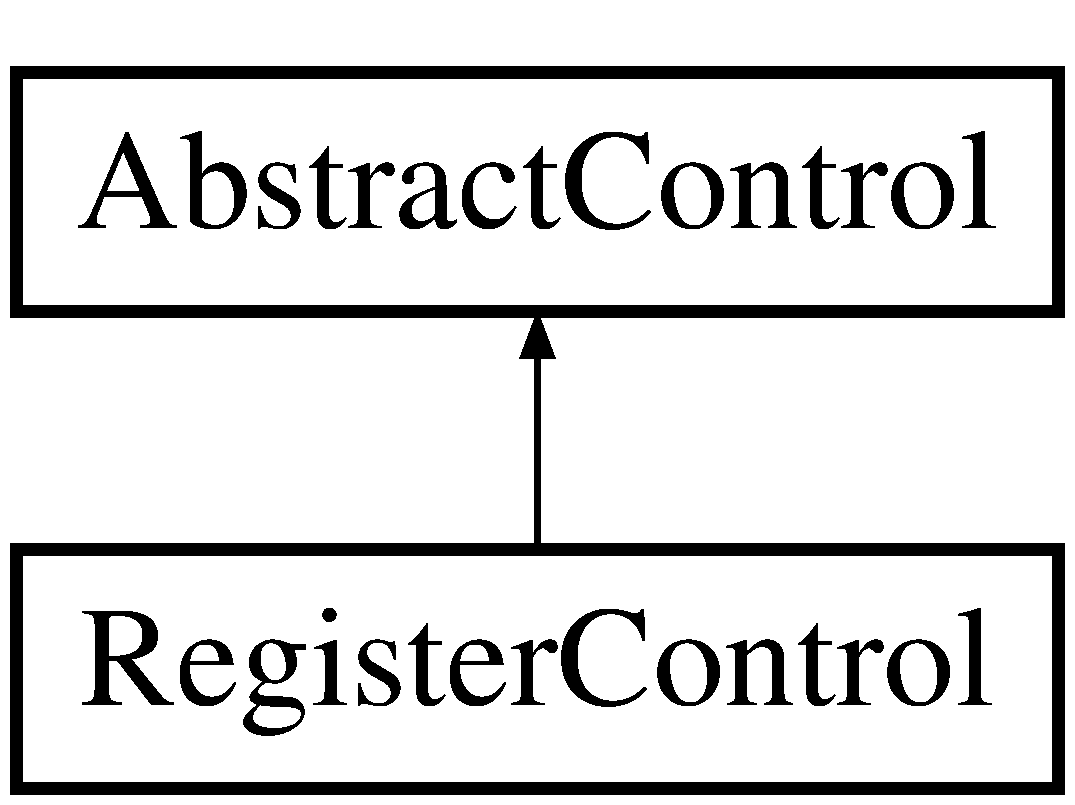
\includegraphics[height=2.000000cm]{class_register_control}
\end{center}
\end{figure}
\subsection*{Public Member Functions}
\begin{DoxyCompactItemize}
\item 
void \mbox{\hyperlink{class_register_control_ad973b13d8abde9fa2a9a0cd623a614b3}{register\+Member}} (Member\+Types type, string name, string security\+Number, string address, string id, string password)
\end{DoxyCompactItemize}
\subsection*{Additional Inherited Members}


\subsection{Member Function Documentation}
\mbox{\Hypertarget{class_register_control_ad973b13d8abde9fa2a9a0cd623a614b3}\label{class_register_control_ad973b13d8abde9fa2a9a0cd623a614b3}} 
\index{Register\+Control@{Register\+Control}!register\+Member@{register\+Member}}
\index{register\+Member@{register\+Member}!Register\+Control@{Register\+Control}}
\subsubsection{\texorpdfstring{register\+Member()}{registerMember()}}
{\footnotesize\ttfamily void Register\+Control\+::register\+Member (\begin{DoxyParamCaption}\item[{Member\+Types}]{type,  }\item[{string}]{name,  }\item[{string}]{security\+Number,  }\item[{string}]{address,  }\item[{string}]{id,  }\item[{string}]{password }\end{DoxyParamCaption})}

회원등록 요청을 수행 
\begin{DoxyParams}{Parameters}
{\em type} & \\
\hline
{\em name} & \\
\hline
{\em security\+Number} & \\
\hline
{\em address} & \\
\hline
{\em id} & \\
\hline
{\em password} & \\
\hline
\end{DoxyParams}


The documentation for this class was generated from the following files\+:\begin{DoxyCompactItemize}
\item 
src/controls/Register\+Control.\+h\item 
src/controls/Register\+Control.\+cpp\end{DoxyCompactItemize}

\hypertarget{class_register_u_i}{}\section{Register\+UI Class Reference}
\label{class_register_u_i}\index{Register\+UI@{Register\+UI}}
Inheritance diagram for Register\+UI\+:\begin{figure}[H]
\begin{center}
\leavevmode
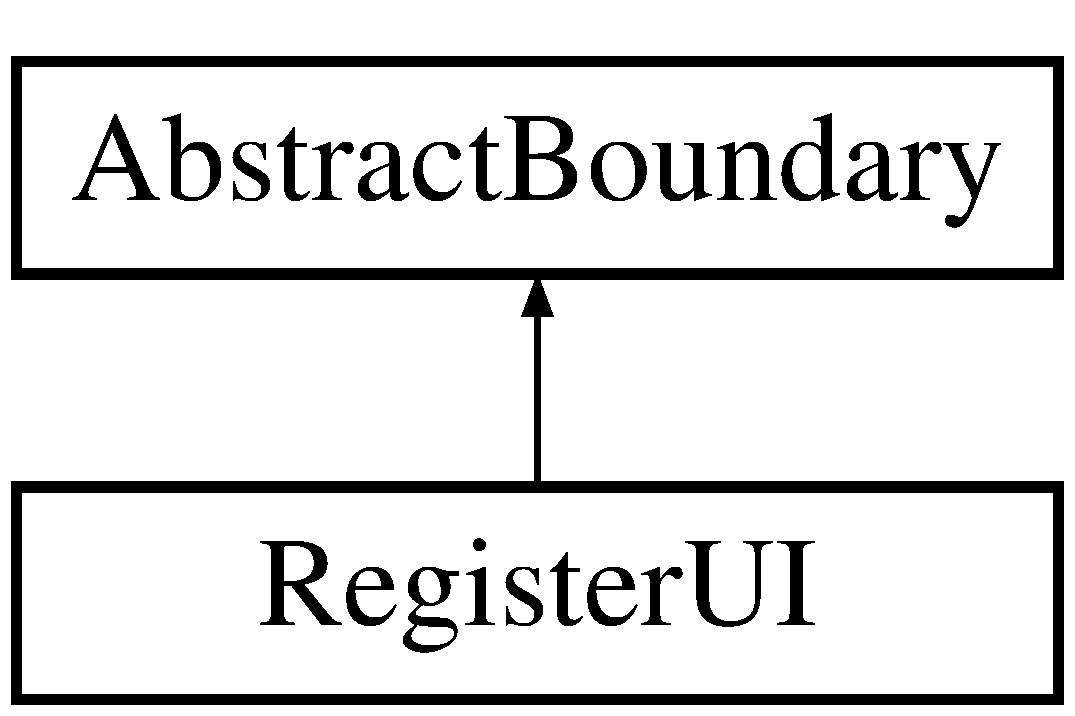
\includegraphics[height=2.000000cm]{class_register_u_i}
\end{center}
\end{figure}
\subsection*{Public Member Functions}
\begin{DoxyCompactItemize}
\item 
\mbox{\Hypertarget{class_register_u_i_aae14cecd8059e2542695140d1b25c30c}\label{class_register_u_i_aae14cecd8059e2542695140d1b25c30c}} 
void {\bfseries on\+Register\+Request} (Member\+Types type, string name, string security\+Number, string address, string id, string password)
\end{DoxyCompactItemize}
\subsection*{Additional Inherited Members}


The documentation for this class was generated from the following files\+:\begin{DoxyCompactItemize}
\item 
src/boundaries/Register\+U\+I.\+h\item 
src/boundaries/Register\+U\+I.\+cpp\end{DoxyCompactItemize}

\hypertarget{class_reservation}{}\section{Reservation Class Reference}
\label{class_reservation}\index{Reservation@{Reservation}}
\subsection*{Public Member Functions}
\begin{DoxyCompactItemize}
\item 
\mbox{\Hypertarget{class_reservation_a4ce6d165547e6b575a0486a43d756cba}\label{class_reservation_a4ce6d165547e6b575a0486a43d756cba}} 
{\bfseries Reservation} (const string \&hostid, const string \&guestid, const string \&name, const string \&address, const string \&date, int cost)
\item 
\mbox{\Hypertarget{class_reservation_a3a17896182f418576039658a70f97452}\label{class_reservation_a3a17896182f418576039658a70f97452}} 
const string \& {\bfseries get\+Guest\+ID} () const
\item 
\mbox{\Hypertarget{class_reservation_ac43be40b51d10a9d2862a323858521d1}\label{class_reservation_ac43be40b51d10a9d2862a323858521d1}} 
void {\bfseries set\+Guesid} (const string \&guesid)
\item 
\mbox{\Hypertarget{class_reservation_a3dbe71a8f1ba4ec469653d305c8a2f28}\label{class_reservation_a3dbe71a8f1ba4ec469653d305c8a2f28}} 
const string \& {\bfseries get\+Host\+ID} () const
\item 
\mbox{\Hypertarget{class_reservation_aaed786c6301ebddfb93fe98e7d4c27c0}\label{class_reservation_aaed786c6301ebddfb93fe98e7d4c27c0}} 
void {\bfseries set\+Hostid} (const string \&hostid)
\item 
\mbox{\Hypertarget{class_reservation_aaf6681475402a5a34ff9dc0e374c42b4}\label{class_reservation_aaf6681475402a5a34ff9dc0e374c42b4}} 
const string \& {\bfseries get\+Name} () const
\item 
\mbox{\Hypertarget{class_reservation_ac0d1a56baec2d31202bbb89b71b78f4f}\label{class_reservation_ac0d1a56baec2d31202bbb89b71b78f4f}} 
void {\bfseries set\+Name} (const string \&name)
\item 
\mbox{\Hypertarget{class_reservation_aaa52ea0877fab25ac0eb37b83ae2a5f3}\label{class_reservation_aaa52ea0877fab25ac0eb37b83ae2a5f3}} 
const string \& {\bfseries get\+Address} () const
\item 
\mbox{\Hypertarget{class_reservation_af54a505ed0d448e5436abf55afb3c15b}\label{class_reservation_af54a505ed0d448e5436abf55afb3c15b}} 
void {\bfseries set\+Address} (const string \&address)
\item 
\mbox{\Hypertarget{class_reservation_a41a54af4ed523eaabf62507b15d4df50}\label{class_reservation_a41a54af4ed523eaabf62507b15d4df50}} 
const string \& {\bfseries get\+Date} () const
\item 
\mbox{\Hypertarget{class_reservation_ab742bc4c1a5e33f7a3ffbf2f9393076d}\label{class_reservation_ab742bc4c1a5e33f7a3ffbf2f9393076d}} 
void {\bfseries set\+Date} (const string \&date)
\item 
\mbox{\Hypertarget{class_reservation_a107d082624892399e930637d32524993}\label{class_reservation_a107d082624892399e930637d32524993}} 
int {\bfseries get\+Cost} () const
\item 
\mbox{\Hypertarget{class_reservation_a54d871fc33a39b60f3b99b20e1bf6880}\label{class_reservation_a54d871fc33a39b60f3b99b20e1bf6880}} 
void {\bfseries set\+Cost} (int cost)
\end{DoxyCompactItemize}


The documentation for this class was generated from the following files\+:\begin{DoxyCompactItemize}
\item 
src/Reservation.\+h\item 
src/Reservation.\+cpp\end{DoxyCompactItemize}

\hypertarget{class_reservation_collection}{}\section{Reservation\+Collection Class Reference}
\label{class_reservation_collection}\index{Reservation\+Collection@{Reservation\+Collection}}
Inheritance diagram for Reservation\+Collection\+:\begin{figure}[H]
\begin{center}
\leavevmode
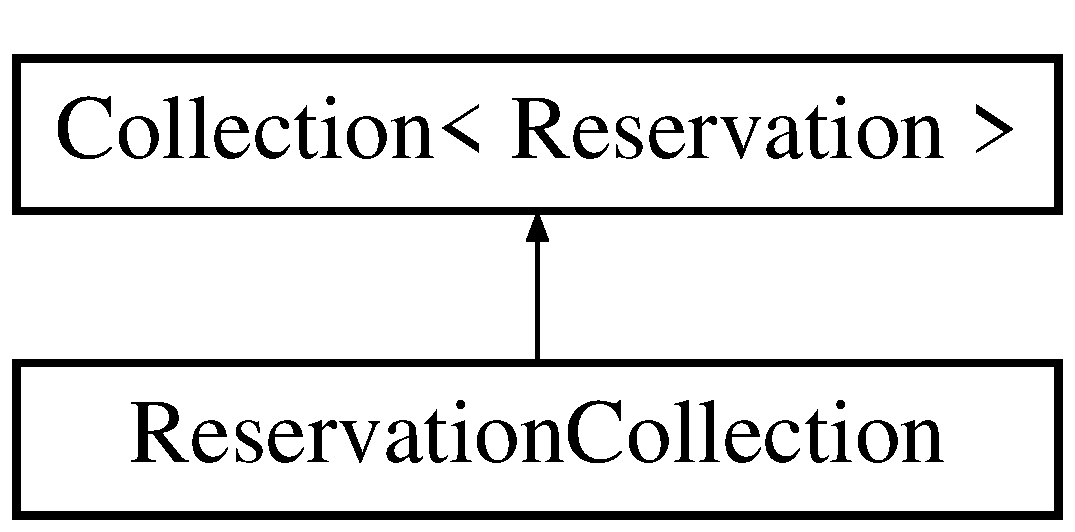
\includegraphics[height=2.000000cm]{class_reservation_collection}
\end{center}
\end{figure}
\subsection*{Additional Inherited Members}


The documentation for this class was generated from the following files\+:\begin{DoxyCompactItemize}
\item 
src/Reservation\+Collection.\+h\item 
src/Reservation\+Collection.\+cpp\end{DoxyCompactItemize}

\hypertarget{class_search_control}{}\section{Search\+Control Class Reference}
\label{class_search_control}\index{Search\+Control@{Search\+Control}}


{\ttfamily \#include $<$Search\+Control.\+h$>$}

Inheritance diagram for Search\+Control\+:\begin{figure}[H]
\begin{center}
\leavevmode
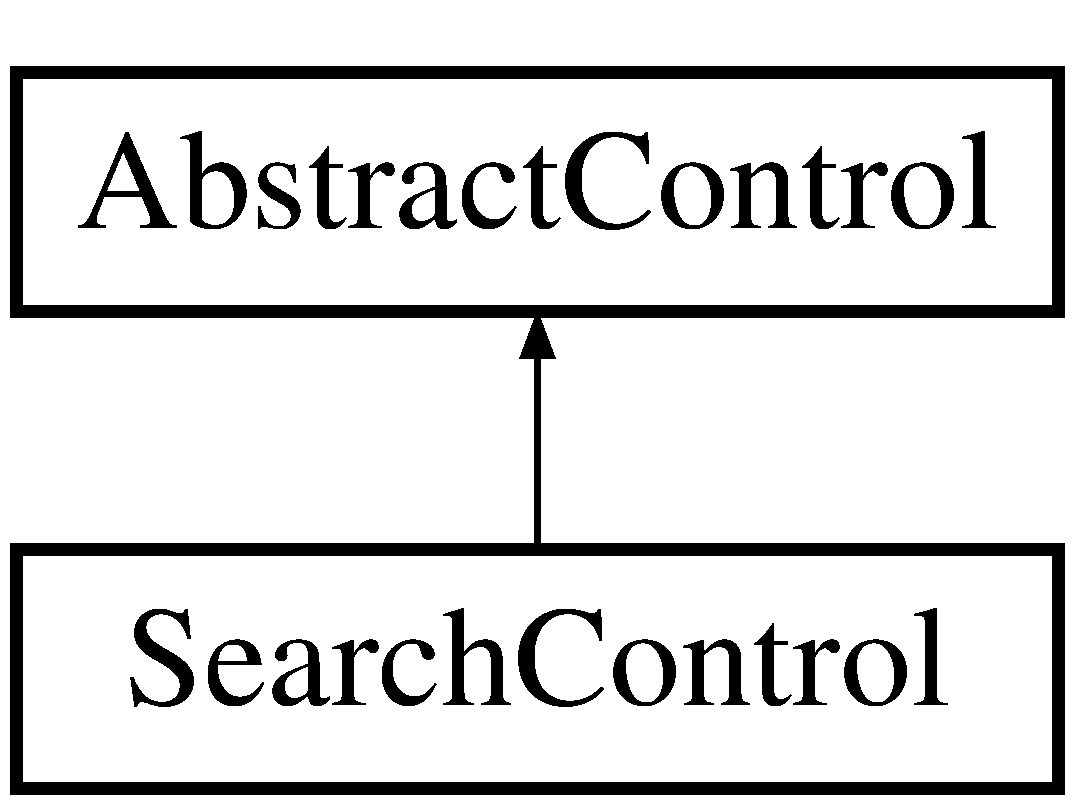
\includegraphics[height=2.000000cm]{class_search_control}
\end{center}
\end{figure}
\subsection*{Public Member Functions}
\begin{DoxyCompactItemize}
\item 
\mbox{\Hypertarget{class_search_control_a96712e21f990caabad392818bd3a17a7}\label{class_search_control_a96712e21f990caabad392818bd3a17a7}} 
void {\bfseries search\+Accommodations} (string address, string date)
\item 
\mbox{\Hypertarget{class_search_control_a754ae7a3d0b00057a559034750422faa}\label{class_search_control_a754ae7a3d0b00057a559034750422faa}} 
void {\bfseries add\+Reservation} (string hostid, string guestid, string accommoname)
\end{DoxyCompactItemize}
\subsection*{Additional Inherited Members}


\subsection{Detailed Description}
숙소 검색 + 예약 시도 

The documentation for this class was generated from the following files\+:\begin{DoxyCompactItemize}
\item 
src/controls/Search\+Control.\+h\item 
src/controls/Search\+Control.\+cpp\end{DoxyCompactItemize}

\hypertarget{class_search_reservation_control}{}\section{Search\+Reservation\+Control Class Reference}
\label{class_search_reservation_control}\index{Search\+Reservation\+Control@{Search\+Reservation\+Control}}


{\ttfamily \#include $<$Search\+Reservation\+Control.\+h$>$}

Inheritance diagram for Search\+Reservation\+Control\+:\begin{figure}[H]
\begin{center}
\leavevmode
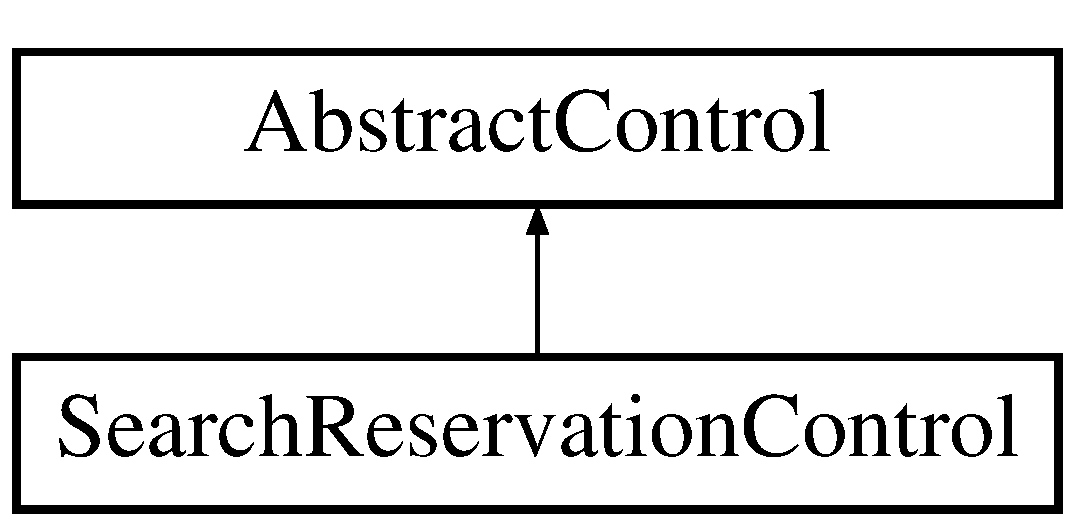
\includegraphics[height=2.000000cm]{class_search_reservation_control}
\end{center}
\end{figure}
\subsection*{Public Member Functions}
\begin{DoxyCompactItemize}
\item 
void \mbox{\hyperlink{class_search_reservation_control_abe42c4bf494cbafebad773f9b0737b98}{Search\+Reservation}} ()
\end{DoxyCompactItemize}
\subsection*{Additional Inherited Members}


\subsection{Detailed Description}
예약 내역 조회 

\subsection{Member Function Documentation}
\mbox{\Hypertarget{class_search_reservation_control_abe42c4bf494cbafebad773f9b0737b98}\label{class_search_reservation_control_abe42c4bf494cbafebad773f9b0737b98}} 
\index{Search\+Reservation\+Control@{Search\+Reservation\+Control}!Search\+Reservation@{Search\+Reservation}}
\index{Search\+Reservation@{Search\+Reservation}!Search\+Reservation\+Control@{Search\+Reservation\+Control}}
\subsubsection{\texorpdfstring{Search\+Reservation()}{SearchReservation()}}
{\footnotesize\ttfamily void Search\+Reservation\+Control\+::\+Search\+Reservation (\begin{DoxyParamCaption}{ }\end{DoxyParamCaption})}

현재 세션의 예약 내역을 list 

The documentation for this class was generated from the following files\+:\begin{DoxyCompactItemize}
\item 
src/controls/Search\+Reservation\+Control.\+h\item 
src/controls/Search\+Reservation\+Control.\+cpp\end{DoxyCompactItemize}

\hypertarget{class_search_reservation_u_i}{}\section{Search\+Reservation\+UI Class Reference}
\label{class_search_reservation_u_i}\index{Search\+Reservation\+UI@{Search\+Reservation\+UI}}
Inheritance diagram for Search\+Reservation\+UI\+:\begin{figure}[H]
\begin{center}
\leavevmode
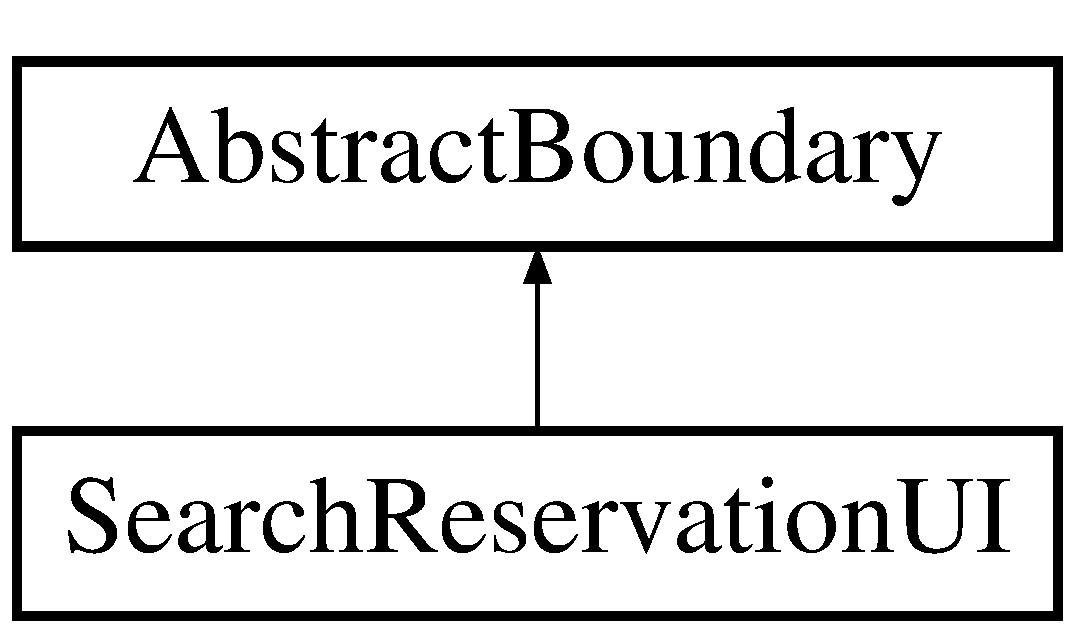
\includegraphics[height=2.000000cm]{class_search_reservation_u_i}
\end{center}
\end{figure}
\subsection*{Public Member Functions}
\begin{DoxyCompactItemize}
\item 
\mbox{\Hypertarget{class_search_reservation_u_i_af97ce0701730415b5ca8dd1d4ee44650}\label{class_search_reservation_u_i_af97ce0701730415b5ca8dd1d4ee44650}} 
void {\bfseries on\+Search\+Reservation\+Request} ()
\end{DoxyCompactItemize}
\subsection*{Additional Inherited Members}


The documentation for this class was generated from the following files\+:\begin{DoxyCompactItemize}
\item 
src/boundaries/Search\+Reservation\+U\+I.\+h\item 
src/boundaries/Search\+Reservation\+U\+I.\+cpp\end{DoxyCompactItemize}

\hypertarget{class_search_u_i}{}\section{Search\+UI Class Reference}
\label{class_search_u_i}\index{Search\+UI@{Search\+UI}}
Inheritance diagram for Search\+UI\+:\begin{figure}[H]
\begin{center}
\leavevmode
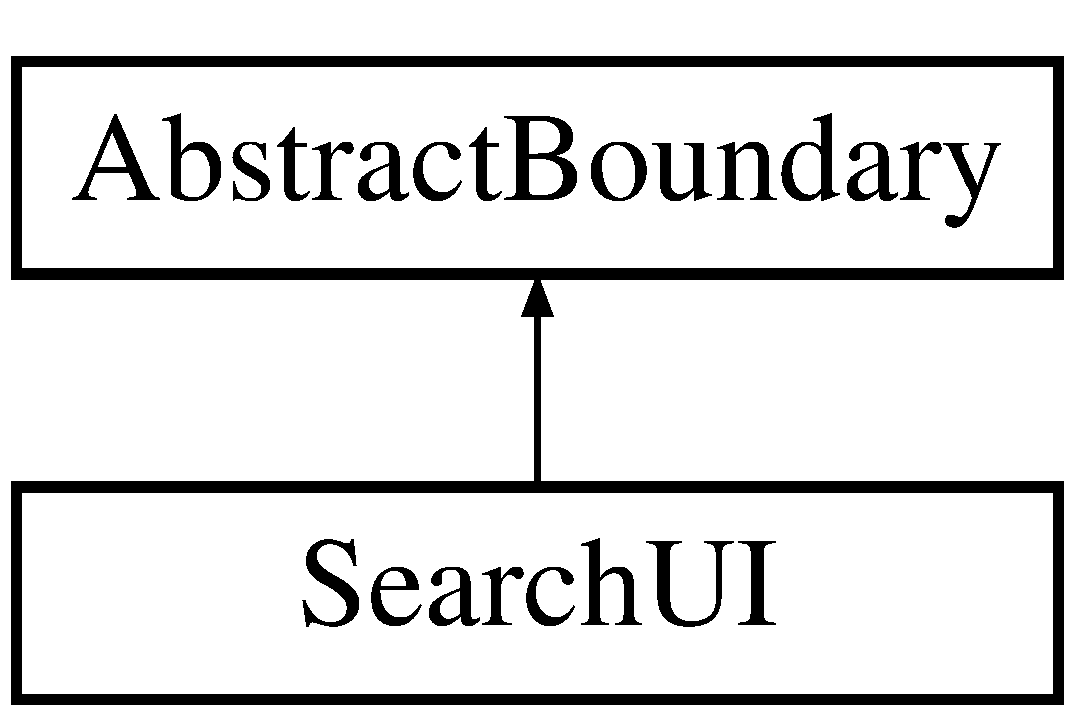
\includegraphics[height=2.000000cm]{class_search_u_i}
\end{center}
\end{figure}
\subsection*{Public Member Functions}
\begin{DoxyCompactItemize}
\item 
void \mbox{\hyperlink{class_search_u_i_adb0e0b5eb6fd7d5d0a98f1eb0239e6d3}{list\+Search\+Result}} (string basic\+\_\+string, string basic\+String)
\item 
void \mbox{\hyperlink{class_search_u_i_a135ce7a4e608e1039612b926b85aac15}{on\+Reservate\+Button\+Click}} (string hostid, string guestid, string accommoname)
\end{DoxyCompactItemize}
\subsection*{Additional Inherited Members}


\subsection{Member Function Documentation}
\mbox{\Hypertarget{class_search_u_i_adb0e0b5eb6fd7d5d0a98f1eb0239e6d3}\label{class_search_u_i_adb0e0b5eb6fd7d5d0a98f1eb0239e6d3}} 
\index{Search\+UI@{Search\+UI}!list\+Search\+Result@{list\+Search\+Result}}
\index{list\+Search\+Result@{list\+Search\+Result}!Search\+UI@{Search\+UI}}
\subsubsection{\texorpdfstring{list\+Search\+Result()}{listSearchResult()}}
{\footnotesize\ttfamily void Search\+U\+I\+::list\+Search\+Result (\begin{DoxyParamCaption}\item[{string}]{basic\+\_\+string,  }\item[{string}]{basic\+String }\end{DoxyParamCaption})}

검색 요청 
\begin{DoxyParams}{Parameters}
{\em basic\+\_\+string} & \\
\hline
{\em basic\+String} & \\
\hline
\end{DoxyParams}
\mbox{\Hypertarget{class_search_u_i_a135ce7a4e608e1039612b926b85aac15}\label{class_search_u_i_a135ce7a4e608e1039612b926b85aac15}} 
\index{Search\+UI@{Search\+UI}!on\+Reservate\+Button\+Click@{on\+Reservate\+Button\+Click}}
\index{on\+Reservate\+Button\+Click@{on\+Reservate\+Button\+Click}!Search\+UI@{Search\+UI}}
\subsubsection{\texorpdfstring{on\+Reservate\+Button\+Click()}{onReservateButtonClick()}}
{\footnotesize\ttfamily void Search\+U\+I\+::on\+Reservate\+Button\+Click (\begin{DoxyParamCaption}\item[{string}]{hostid,  }\item[{string}]{guestid,  }\item[{string}]{accommoname }\end{DoxyParamCaption})}

예약 시도 
\begin{DoxyParams}{Parameters}
{\em hostid} & \\
\hline
{\em guestid} & \\
\hline
{\em accommoname} & \\
\hline
\end{DoxyParams}


The documentation for this class was generated from the following files\+:\begin{DoxyCompactItemize}
\item 
src/boundaries/Search\+U\+I.\+h\item 
src/boundaries/Search\+U\+I.\+cpp\end{DoxyCompactItemize}

\hypertarget{class_session}{}\section{Session Class Reference}
\label{class_session}\index{Session@{Session}}
\subsection*{Public Member Functions}
\begin{DoxyCompactItemize}
\item 
\mbox{\hyperlink{class_session_ad92ef09b872c9227e38a6efdd4d8a837}{Session}} ()
\item 
\mbox{\hyperlink{class_session_a7f366328741cdcd4200f3184c85d507a}{Session}} (\mbox{\hyperlink{class_member}{Member}} $\ast$member)
\item 
\mbox{\Hypertarget{class_session_aeae3ee95ffc22efdca7112eb10f84c4d}\label{class_session_aeae3ee95ffc22efdca7112eb10f84c4d}} 
bool {\bfseries is\+Guest} ()
\item 
\mbox{\Hypertarget{class_session_a4867a03de74afef38b440ba32bee98ab}\label{class_session_a4867a03de74afef38b440ba32bee98ab}} 
\mbox{\hyperlink{class_member}{Member}} $\ast$ {\bfseries get\+Member} ()
\end{DoxyCompactItemize}


\subsection{Constructor \& Destructor Documentation}
\mbox{\Hypertarget{class_session_ad92ef09b872c9227e38a6efdd4d8a837}\label{class_session_ad92ef09b872c9227e38a6efdd4d8a837}} 
\index{Session@{Session}!Session@{Session}}
\index{Session@{Session}!Session@{Session}}
\subsubsection{\texorpdfstring{Session()}{Session()}\hspace{0.1cm}{\footnotesize\ttfamily [1/2]}}
{\footnotesize\ttfamily Session\+::\+Session (\begin{DoxyParamCaption}{ }\end{DoxyParamCaption})}

\mbox{\hyperlink{class_guest}{Guest}} 세션 생성자. \mbox{\Hypertarget{class_session_a7f366328741cdcd4200f3184c85d507a}\label{class_session_a7f366328741cdcd4200f3184c85d507a}} 
\index{Session@{Session}!Session@{Session}}
\index{Session@{Session}!Session@{Session}}
\subsubsection{\texorpdfstring{Session()}{Session()}\hspace{0.1cm}{\footnotesize\ttfamily [2/2]}}
{\footnotesize\ttfamily Session\+::\+Session (\begin{DoxyParamCaption}\item[{\mbox{\hyperlink{class_member}{Member}} $\ast$}]{member }\end{DoxyParamCaption})}

로그인 사용자 세션 
\begin{DoxyParams}{Parameters}
{\em member} & \\
\hline
\end{DoxyParams}


The documentation for this class was generated from the following files\+:\begin{DoxyCompactItemize}
\item 
src/Session.\+h\item 
src/Session.\+cpp\end{DoxyCompactItemize}

\hypertarget{class_session_collection}{}\section{Session\+Collection Class Reference}
\label{class_session_collection}\index{Session\+Collection@{Session\+Collection}}


{\ttfamily \#include $<$Session\+Collection.\+h$>$}

Inheritance diagram for Session\+Collection\+:\begin{figure}[H]
\begin{center}
\leavevmode
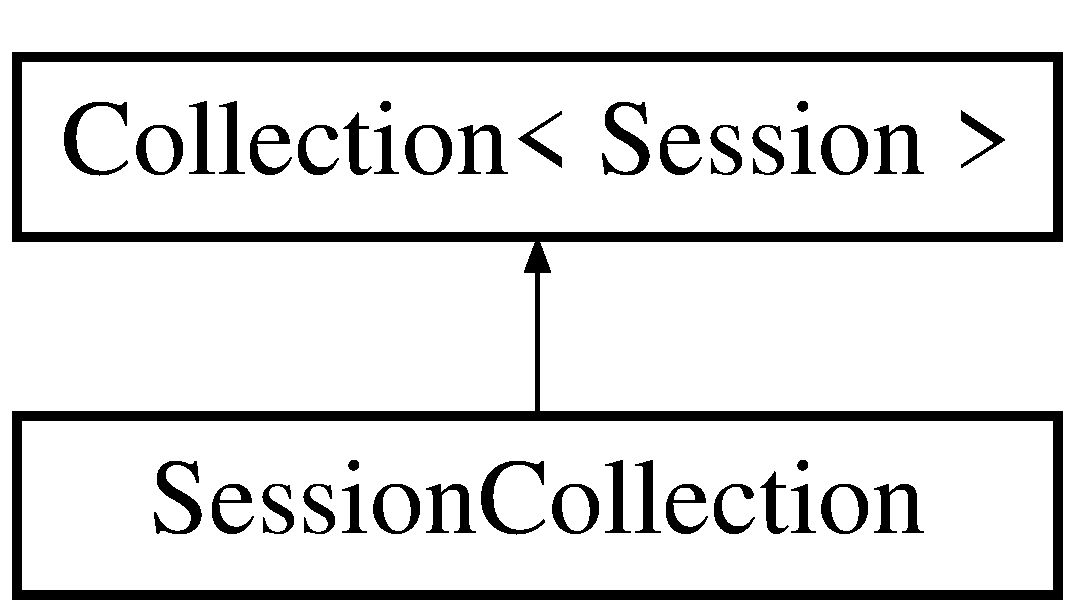
\includegraphics[height=2.000000cm]{class_session_collection}
\end{center}
\end{figure}
\subsection*{Public Member Functions}
\begin{DoxyCompactItemize}
\item 
\mbox{\Hypertarget{class_session_collection_a57ca0e2003ebc212dc0179c80201b3d1}\label{class_session_collection_a57ca0e2003ebc212dc0179c80201b3d1}} 
\mbox{\hyperlink{class_session}{Session}} $\ast$ {\bfseries get\+Current\+Session} () const
\item 
bool \mbox{\hyperlink{class_session_collection_a52b76b5e700a4b3395784bbe56ccd1c4}{change\+Current\+Session}} (\mbox{\hyperlink{class_session}{Session}} $\ast$)
\item 
bool \mbox{\hyperlink{class_session_collection_a516c5d275d9adc47040c5acbe1e47372}{change\+Current\+Session}} (string user\+ID)
\item 
void \mbox{\hyperlink{class_session_collection_ada1aab5737803b2f9b11d91c412d8047}{change\+Current\+Session\+To\+Guest}} ()
\end{DoxyCompactItemize}
\subsection*{Additional Inherited Members}


\subsection{Detailed Description}
\mbox{\hyperlink{class_session}{Session}} \mbox{\hyperlink{class_collection}{Collection}} 현재 로그인한 모든 사용자의 세션들과 \mbox{\hyperlink{class_guest}{Guest}} 세션을 가지고있다. collection내에 \mbox{\hyperlink{class_guest}{Guest}} 세션은 반드시 하나만 존재한다. 

\subsection{Member Function Documentation}
\mbox{\Hypertarget{class_session_collection_a52b76b5e700a4b3395784bbe56ccd1c4}\label{class_session_collection_a52b76b5e700a4b3395784bbe56ccd1c4}} 
\index{Session\+Collection@{Session\+Collection}!change\+Current\+Session@{change\+Current\+Session}}
\index{change\+Current\+Session@{change\+Current\+Session}!Session\+Collection@{Session\+Collection}}
\subsubsection{\texorpdfstring{change\+Current\+Session()}{changeCurrentSession()}\hspace{0.1cm}{\footnotesize\ttfamily [1/2]}}
{\footnotesize\ttfamily bool Session\+Collection\+::change\+Current\+Session (\begin{DoxyParamCaption}\item[{\mbox{\hyperlink{class_session}{Session}} $\ast$}]{session }\end{DoxyParamCaption})}

현재 세션을 변경한다. \begin{DoxyReturn}{Returns}
변경 성공 여부 
\end{DoxyReturn}
\mbox{\Hypertarget{class_session_collection_a516c5d275d9adc47040c5acbe1e47372}\label{class_session_collection_a516c5d275d9adc47040c5acbe1e47372}} 
\index{Session\+Collection@{Session\+Collection}!change\+Current\+Session@{change\+Current\+Session}}
\index{change\+Current\+Session@{change\+Current\+Session}!Session\+Collection@{Session\+Collection}}
\subsubsection{\texorpdfstring{change\+Current\+Session()}{changeCurrentSession()}\hspace{0.1cm}{\footnotesize\ttfamily [2/2]}}
{\footnotesize\ttfamily bool Session\+Collection\+::change\+Current\+Session (\begin{DoxyParamCaption}\item[{string}]{user\+ID }\end{DoxyParamCaption})}

현재 세션을 id=\{user\+ID\} 사용자의 세션으로 변경한다. 
\begin{DoxyParams}{Parameters}
{\em user\+ID} & 사용자\+ID \\
\hline
\end{DoxyParams}
\begin{DoxyReturn}{Returns}
변경 성공 여부 
\end{DoxyReturn}
\mbox{\Hypertarget{class_session_collection_ada1aab5737803b2f9b11d91c412d8047}\label{class_session_collection_ada1aab5737803b2f9b11d91c412d8047}} 
\index{Session\+Collection@{Session\+Collection}!change\+Current\+Session\+To\+Guest@{change\+Current\+Session\+To\+Guest}}
\index{change\+Current\+Session\+To\+Guest@{change\+Current\+Session\+To\+Guest}!Session\+Collection@{Session\+Collection}}
\subsubsection{\texorpdfstring{change\+Current\+Session\+To\+Guest()}{changeCurrentSessionToGuest()}}
{\footnotesize\ttfamily void Session\+Collection\+::change\+Current\+Session\+To\+Guest (\begin{DoxyParamCaption}{ }\end{DoxyParamCaption})}

현재 세션을 \mbox{\hyperlink{class_guest}{Guest}} 세션으로 변경한다. 

The documentation for this class was generated from the following files\+:\begin{DoxyCompactItemize}
\item 
src/Session\+Collection.\+h\item 
src/Session\+Collection.\+cpp\end{DoxyCompactItemize}

\hypertarget{class_session_control}{}\section{Session\+Control Class Reference}
\label{class_session_control}\index{Session\+Control@{Session\+Control}}


{\ttfamily \#include $<$Session\+Control.\+h$>$}

Inheritance diagram for Session\+Control\+:\begin{figure}[H]
\begin{center}
\leavevmode
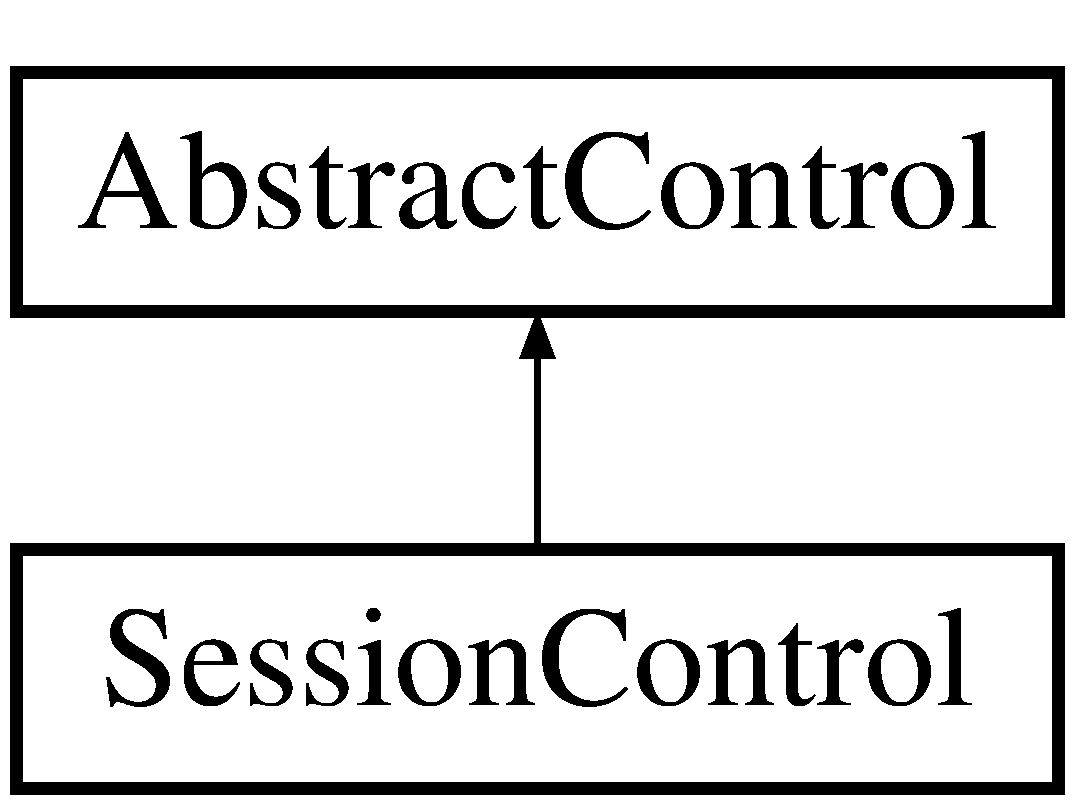
\includegraphics[height=2.000000cm]{class_session_control}
\end{center}
\end{figure}
\subsection*{Public Member Functions}
\begin{DoxyCompactItemize}
\item 
void \mbox{\hyperlink{class_session_control_a09ae13f1e995c6b83ece478921c0722f}{change\+Session}} (string user\+ID)
\item 
void \mbox{\hyperlink{class_session_control_a2b5ea3cfba3e5f303071845330a69069}{change\+Session\+To\+Guest}} ()
\end{DoxyCompactItemize}
\subsection*{Additional Inherited Members}


\subsection{Detailed Description}
세션 관련 명령을 수행 

\subsection{Member Function Documentation}
\mbox{\Hypertarget{class_session_control_a09ae13f1e995c6b83ece478921c0722f}\label{class_session_control_a09ae13f1e995c6b83ece478921c0722f}} 
\index{Session\+Control@{Session\+Control}!change\+Session@{change\+Session}}
\index{change\+Session@{change\+Session}!Session\+Control@{Session\+Control}}
\subsubsection{\texorpdfstring{change\+Session()}{changeSession()}}
{\footnotesize\ttfamily void Session\+Control\+::change\+Session (\begin{DoxyParamCaption}\item[{string}]{user\+ID }\end{DoxyParamCaption})}

세션 전환 
\begin{DoxyParams}{Parameters}
{\em user\+ID} & \\
\hline
\end{DoxyParams}
\mbox{\Hypertarget{class_session_control_a2b5ea3cfba3e5f303071845330a69069}\label{class_session_control_a2b5ea3cfba3e5f303071845330a69069}} 
\index{Session\+Control@{Session\+Control}!change\+Session\+To\+Guest@{change\+Session\+To\+Guest}}
\index{change\+Session\+To\+Guest@{change\+Session\+To\+Guest}!Session\+Control@{Session\+Control}}
\subsubsection{\texorpdfstring{change\+Session\+To\+Guest()}{changeSessionToGuest()}}
{\footnotesize\ttfamily void Session\+Control\+::change\+Session\+To\+Guest (\begin{DoxyParamCaption}{ }\end{DoxyParamCaption})}

\mbox{\hyperlink{class_guest}{Guest}} 세션 전환 

The documentation for this class was generated from the following files\+:\begin{DoxyCompactItemize}
\item 
src/controls/Session\+Control.\+h\item 
src/controls/Session\+Control.\+cpp\end{DoxyCompactItemize}

\hypertarget{class_session_u_i}{}\section{Session\+UI Class Reference}
\label{class_session_u_i}\index{Session\+UI@{Session\+UI}}
Inheritance diagram for Session\+UI\+:\begin{figure}[H]
\begin{center}
\leavevmode
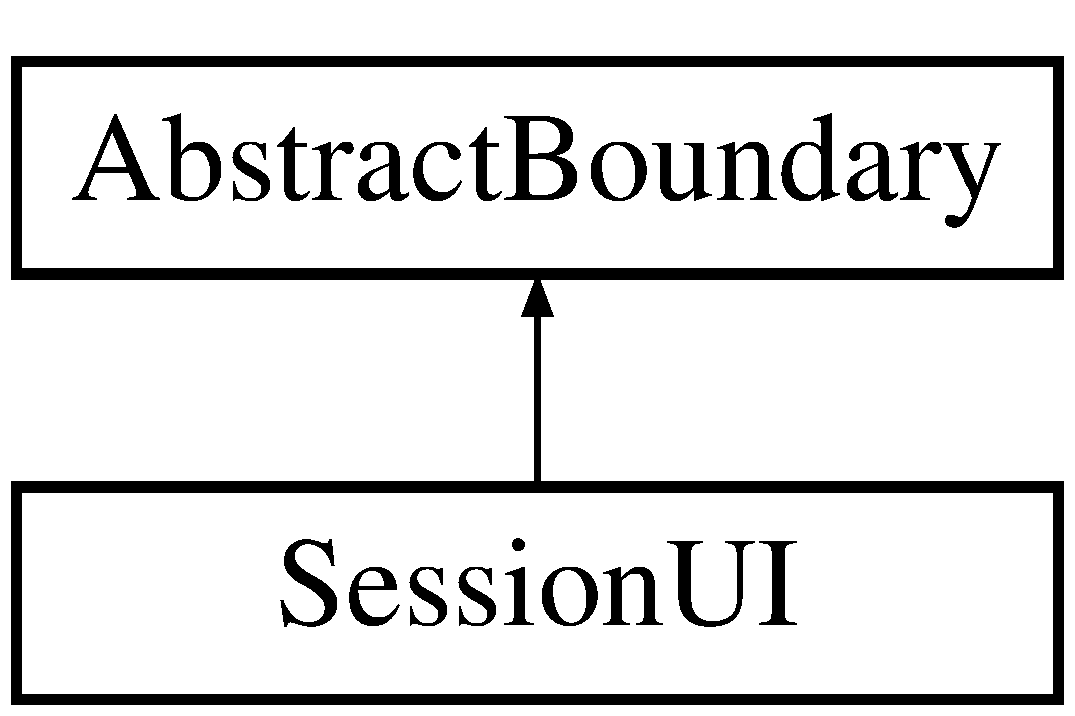
\includegraphics[height=2.000000cm]{class_session_u_i}
\end{center}
\end{figure}
\subsection*{Public Member Functions}
\begin{DoxyCompactItemize}
\item 
\mbox{\Hypertarget{class_session_u_i_a32778b6a6b4323e9c067b37903906fcf}\label{class_session_u_i_a32778b6a6b4323e9c067b37903906fcf}} 
void {\bfseries on\+Change\+Session} (char $\ast$)
\item 
\mbox{\Hypertarget{class_session_u_i_a9d92daa17c05d5c2eaf13a53b9edf13d}\label{class_session_u_i_a9d92daa17c05d5c2eaf13a53b9edf13d}} 
void {\bfseries on\+Change\+Guest\+Session} ()
\end{DoxyCompactItemize}
\subsection*{Additional Inherited Members}


The documentation for this class was generated from the following files\+:\begin{DoxyCompactItemize}
\item 
src/boundaries/Session\+U\+I.\+h\item 
src/boundaries/Session\+U\+I.\+cpp\end{DoxyCompactItemize}

\hypertarget{class_time}{}\section{Time Class Reference}
\label{class_time}\index{Time@{Time}}
\subsection*{Static Public Member Functions}
\begin{DoxyCompactItemize}
\item 
\mbox{\Hypertarget{class_time_a01febf5c2528829c56eca9abbda9974a}\label{class_time_a01febf5c2528829c56eca9abbda9974a}} 
static void {\bfseries set\+Current\+Time} (string time)
\item 
\mbox{\Hypertarget{class_time_ab6e399daf85a2a3f2b69aa0715201930}\label{class_time_ab6e399daf85a2a3f2b69aa0715201930}} 
static string {\bfseries get\+Current\+Time} ()
\end{DoxyCompactItemize}


The documentation for this class was generated from the following files\+:\begin{DoxyCompactItemize}
\item 
src/Time.\+h\item 
src/Time.\+cpp\end{DoxyCompactItemize}

\hypertarget{class_withdrawal_control}{}\section{Withdrawal\+Control Class Reference}
\label{class_withdrawal_control}\index{Withdrawal\+Control@{Withdrawal\+Control}}


{\ttfamily \#include $<$Withdrawal\+Control.\+h$>$}

Inheritance diagram for Withdrawal\+Control\+:\begin{figure}[H]
\begin{center}
\leavevmode
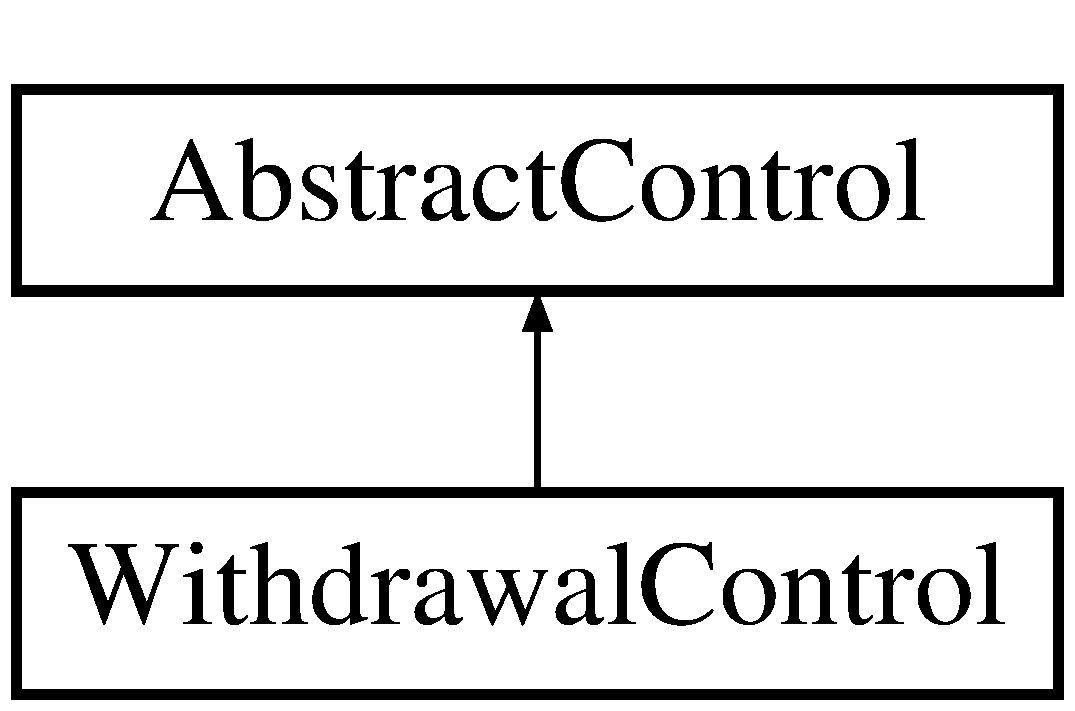
\includegraphics[height=2.000000cm]{class_withdrawal_control}
\end{center}
\end{figure}
\subsection*{Public Member Functions}
\begin{DoxyCompactItemize}
\item 
void \mbox{\hyperlink{class_withdrawal_control_a9bbb9752138ece8a770211cd4d1be5b9}{delete\+Member}} ()
\end{DoxyCompactItemize}
\subsection*{Additional Inherited Members}


\subsection{Detailed Description}
회원 탈퇴 Control 

\subsection{Member Function Documentation}
\mbox{\Hypertarget{class_withdrawal_control_a9bbb9752138ece8a770211cd4d1be5b9}\label{class_withdrawal_control_a9bbb9752138ece8a770211cd4d1be5b9}} 
\index{Withdrawal\+Control@{Withdrawal\+Control}!delete\+Member@{delete\+Member}}
\index{delete\+Member@{delete\+Member}!Withdrawal\+Control@{Withdrawal\+Control}}
\subsubsection{\texorpdfstring{delete\+Member()}{deleteMember()}}
{\footnotesize\ttfamily void Withdrawal\+Control\+::delete\+Member (\begin{DoxyParamCaption}{ }\end{DoxyParamCaption})}

회원 삭제 요청을 수행 

The documentation for this class was generated from the following files\+:\begin{DoxyCompactItemize}
\item 
src/controls/Withdrawal\+Control.\+h\item 
src/controls/Withdrawal\+Control.\+cpp\end{DoxyCompactItemize}

\hypertarget{class_withdrawal_u_i}{}\section{Withdrawal\+UI Class Reference}
\label{class_withdrawal_u_i}\index{Withdrawal\+UI@{Withdrawal\+UI}}
Inheritance diagram for Withdrawal\+UI\+:\begin{figure}[H]
\begin{center}
\leavevmode
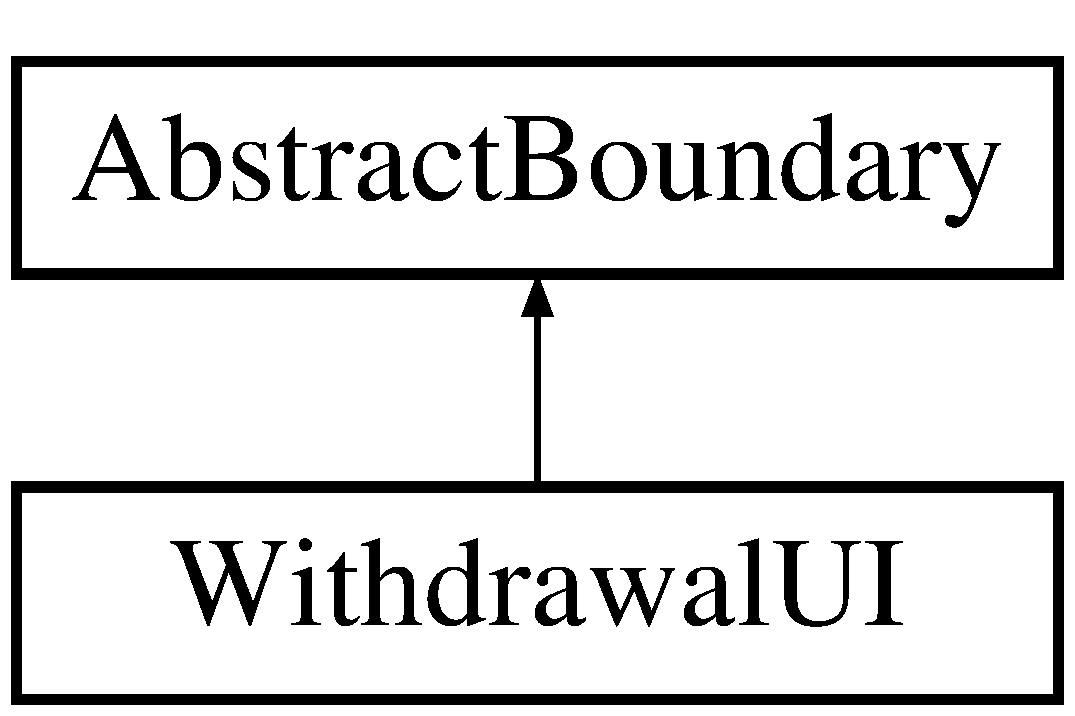
\includegraphics[height=2.000000cm]{class_withdrawal_u_i}
\end{center}
\end{figure}
\subsection*{Public Member Functions}
\begin{DoxyCompactItemize}
\item 
\mbox{\Hypertarget{class_withdrawal_u_i_a3d555adf9eac49498001d9bed12bdbfe}\label{class_withdrawal_u_i_a3d555adf9eac49498001d9bed12bdbfe}} 
void {\bfseries on\+Withdrawal\+Request} ()
\end{DoxyCompactItemize}
\subsection*{Additional Inherited Members}


The documentation for this class was generated from the following files\+:\begin{DoxyCompactItemize}
\item 
src/boundaries/Withdrawal\+U\+I.\+h\item 
src/boundaries/Withdrawal\+U\+I.\+cpp\end{DoxyCompactItemize}

%--- End generated contents ---

% Index
\backmatter
\newpage
\phantomsection
\clearemptydoublepage
\addcontentsline{toc}{chapter}{Index}
\printindex

\end{document}
